% Options for packages loaded elsewhere
\PassOptionsToPackage{unicode}{hyperref}
\PassOptionsToPackage{hyphens}{url}
%
\documentclass[
  10pt,
  ignorenonframetext,
  m]{beamer}
\usepackage{pgfpages}
\setbeamertemplate{caption}[numbered]
\setbeamertemplate{caption label separator}{: }
\setbeamercolor{caption name}{fg=normal text.fg}
\beamertemplatenavigationsymbolsempty
% Prevent slide breaks in the middle of a paragraph
\widowpenalties 1 10000
\raggedbottom
\setbeamertemplate{part page}{
  \centering
  \begin{beamercolorbox}[sep=16pt,center]{part title}
    \usebeamerfont{part title}\insertpart\par
  \end{beamercolorbox}
}
\setbeamertemplate{section page}{
  \centering
  \begin{beamercolorbox}[sep=12pt,center]{part title}
    \usebeamerfont{section title}\insertsection\par
  \end{beamercolorbox}
}
\setbeamertemplate{subsection page}{
  \centering
  \begin{beamercolorbox}[sep=8pt,center]{part title}
    \usebeamerfont{subsection title}\insertsubsection\par
  \end{beamercolorbox}
}
\AtBeginPart{
  \frame{\partpage}
}
\AtBeginSection{
  \ifbibliography
  \else
    \frame{\sectionpage}
  \fi
}
\AtBeginSubsection{
  \frame{\subsectionpage}
}
\usepackage{lmodern}
\usepackage{amssymb,amsmath}
\usepackage{ifxetex,ifluatex}
\ifnum 0\ifxetex 1\fi\ifluatex 1\fi=0 % if pdftex
  \usepackage[T1]{fontenc}
  \usepackage[utf8]{inputenc}
  \usepackage{textcomp} % provide euro and other symbols
\else % if luatex or xetex
  \usepackage{unicode-math}
  \defaultfontfeatures{Scale=MatchLowercase}
  \defaultfontfeatures[\rmfamily]{Ligatures=TeX,Scale=1}
\fi
% Use upquote if available, for straight quotes in verbatim environments
\IfFileExists{upquote.sty}{\usepackage{upquote}}{}
\IfFileExists{microtype.sty}{% use microtype if available
  \usepackage[]{microtype}
  \UseMicrotypeSet[protrusion]{basicmath} % disable protrusion for tt fonts
}{}
\makeatletter
\@ifundefined{KOMAClassName}{% if non-KOMA class
  \IfFileExists{parskip.sty}{%
    \usepackage{parskip}
  }{% else
    \setlength{\parindent}{0pt}
    \setlength{\parskip}{6pt plus 2pt minus 1pt}}
}{% if KOMA class
  \KOMAoptions{parskip=half}}
\makeatother
\usepackage{xcolor}
\IfFileExists{xurl.sty}{\usepackage{xurl}}{} % add URL line breaks if available
\IfFileExists{bookmark.sty}{\usepackage{bookmark}}{\usepackage{hyperref}}
\hypersetup{
  pdftitle={Tools and statistical approaches for integrating DNA sequencing into clinical care},
  pdfauthor={Dayne L Filer},
  hidelinks,
  pdfcreator={LaTeX via pandoc}}
\urlstyle{same} % disable monospaced font for URLs
\newif\ifbibliography
\usepackage{graphicx,grffile}
\makeatletter
\def\maxwidth{\ifdim\Gin@nat@width>\linewidth\linewidth\else\Gin@nat@width\fi}
\def\maxheight{\ifdim\Gin@nat@height>\textheight\textheight\else\Gin@nat@height\fi}
\makeatother
% Scale images if necessary, so that they will not overflow the page
% margins by default, and it is still possible to overwrite the defaults
% using explicit options in \includegraphics[width, height, ...]{}
\setkeys{Gin}{width=\maxwidth,height=\maxheight,keepaspectratio}
% Set default figure placement to htbp
\makeatletter
\def\fps@figure{htbp}
\makeatother
\setlength{\emergencystretch}{3em} % prevent overfull lines
\providecommand{\tightlist}{%
  \setlength{\itemsep}{0pt}\setlength{\parskip}{0pt}}
\setcounter{secnumdepth}{-\maxdimen} % remove section numbering
\usepackage{graphicx}
\usepackage{rotating}
\usepackage{hyperref}
\usepackage{caption}
\usepackage{wasysym}
\usepackage{amsmath}
\usepackage{bm}
\usepackage{multicol}

%% For kableExtra
\usepackage{booktabs}
\usepackage{longtable}
\usepackage{array}
\usepackage{multirow}
\usepackage{wrapfig}
\usepackage{float}
\usepackage{colortbl}
\usepackage{pdflscape}
\usepackage{tabu}
\usepackage{threeparttable} 
\usepackage{threeparttablex} 
\usepackage[normalem]{ulem} 
\usepackage{makecell}
\usepackage{xcolor}

\usetheme[numbering=none]{metropolis}

\institute{
Department of Genetics, Curriculum in Bioinformatics \& Computational Biology \\
Renaissance Computing Institute
}

\setbeamertemplate{title page}[empty]
% \setbeamertemplate{navigation symbols}{%
% \hyperlink{apptoc}{\beamerbutton{*}}
% }
\setbeamertemplate{footline}{%
  \begin{beamercolorbox}[wd=\textwidth, sep=3ex]{footline}%
    \usebeamerfont{page number in head/foot}%
    \usebeamertemplate*{frame footer}
    \hfill%
    \hyperlink{maintoc}{\textcolor{uncnavy}{{$\in$}}}
    \hyperlink{apptoc}{\textcolor{uncnavy}{{$\ni$}}}
  \end{beamercolorbox}%
}
% \titlegraphic{\vspace{4cm}\flushright
\includegraphics[width=0.3\textwidth]{RENCI-logo.png}}

\definecolor{uncblue}{HTML}{4B9CD3}
\definecolor{uncnavy}{HTML}{13294B}
\definecolor{uncblck}{HTML}{151515}
\definecolor{uncgray}{HTML}{F8F8F8}
\definecolor{gray85}{HTML}{D9D9D9}

% \setbeamercolor{palette primary}{fg=uncblue}
% \setbeamercolor{palette secondary}{fg=uncnavy}
% \setbeamercolor{palette tertiary}{fg=uncblue}
% \setbeamercolor{palette quaternary}{fg=uncblue}
% \setbeamercolor{separation line}{fg=uncblue}
\setbeamercolor{progress bar}{fg=uncblue,bg=uncnavy}
\setbeamercolor{frametitle}{fg=uncnavy,bg=uncblue}
\setbeamercolor{title}{fg=uncnavy,bg=uncgray}
\setbeamercolor{local structure}{fg=uncblue}
\setbeamercolor{normal text}{fg=uncblck,bg=uncgray}
\setbeamercolor{section in toc}{fg=uncblue,bg=uncgray}
\setbeamercolor{item projected}{fg=uncblue,bg=uncgray}
% \setbeamercolor{title separator}{fg=uncblue,bg=uncgray}

\setbeamertemplate{itemize item}{\color{uncblue}$\bullet$}
\setbeamertemplate{itemize subitem}{\color{uncblue}\textbf{-}}

\let\Tiny=\tiny

\AtBeginPart{}
\AtBeginSubsection{}
\AtBeginSubsubsection{}
\setlength{\emergencystretch}{0em}
\setlength{\parskip}{0pt}

\title{Tools and statistical approaches for integrating DNA sequencing into
clinical care}
\subtitle{Doctorate of Philosophy Dissertation Defense}
\author{Dayne L Filer}
\date{Monday, November 16 2020}

\begin{document}
\frame{\titlepage}

\begin{frame}{Talk Outline}
\protect\hypertarget{talk-outline}{}

\label{maintoc} \tableofcontents

\end{frame}

\hypertarget{one-minute-primer-on-human-genetics}{%
\section{One-minute primer on human
genetics}\label{one-minute-primer-on-human-genetics}}

\hypertarget{genetic-material-organized-into-chromosomes}{%
\subsection{Genetic material organized into
chromosomes}\label{genetic-material-organized-into-chromosomes}}

\begin{frame}{Genetic material organized into chromosomes}
\protect\hypertarget{genetic-material-organized-into-chromosomes-1}{}

\centering

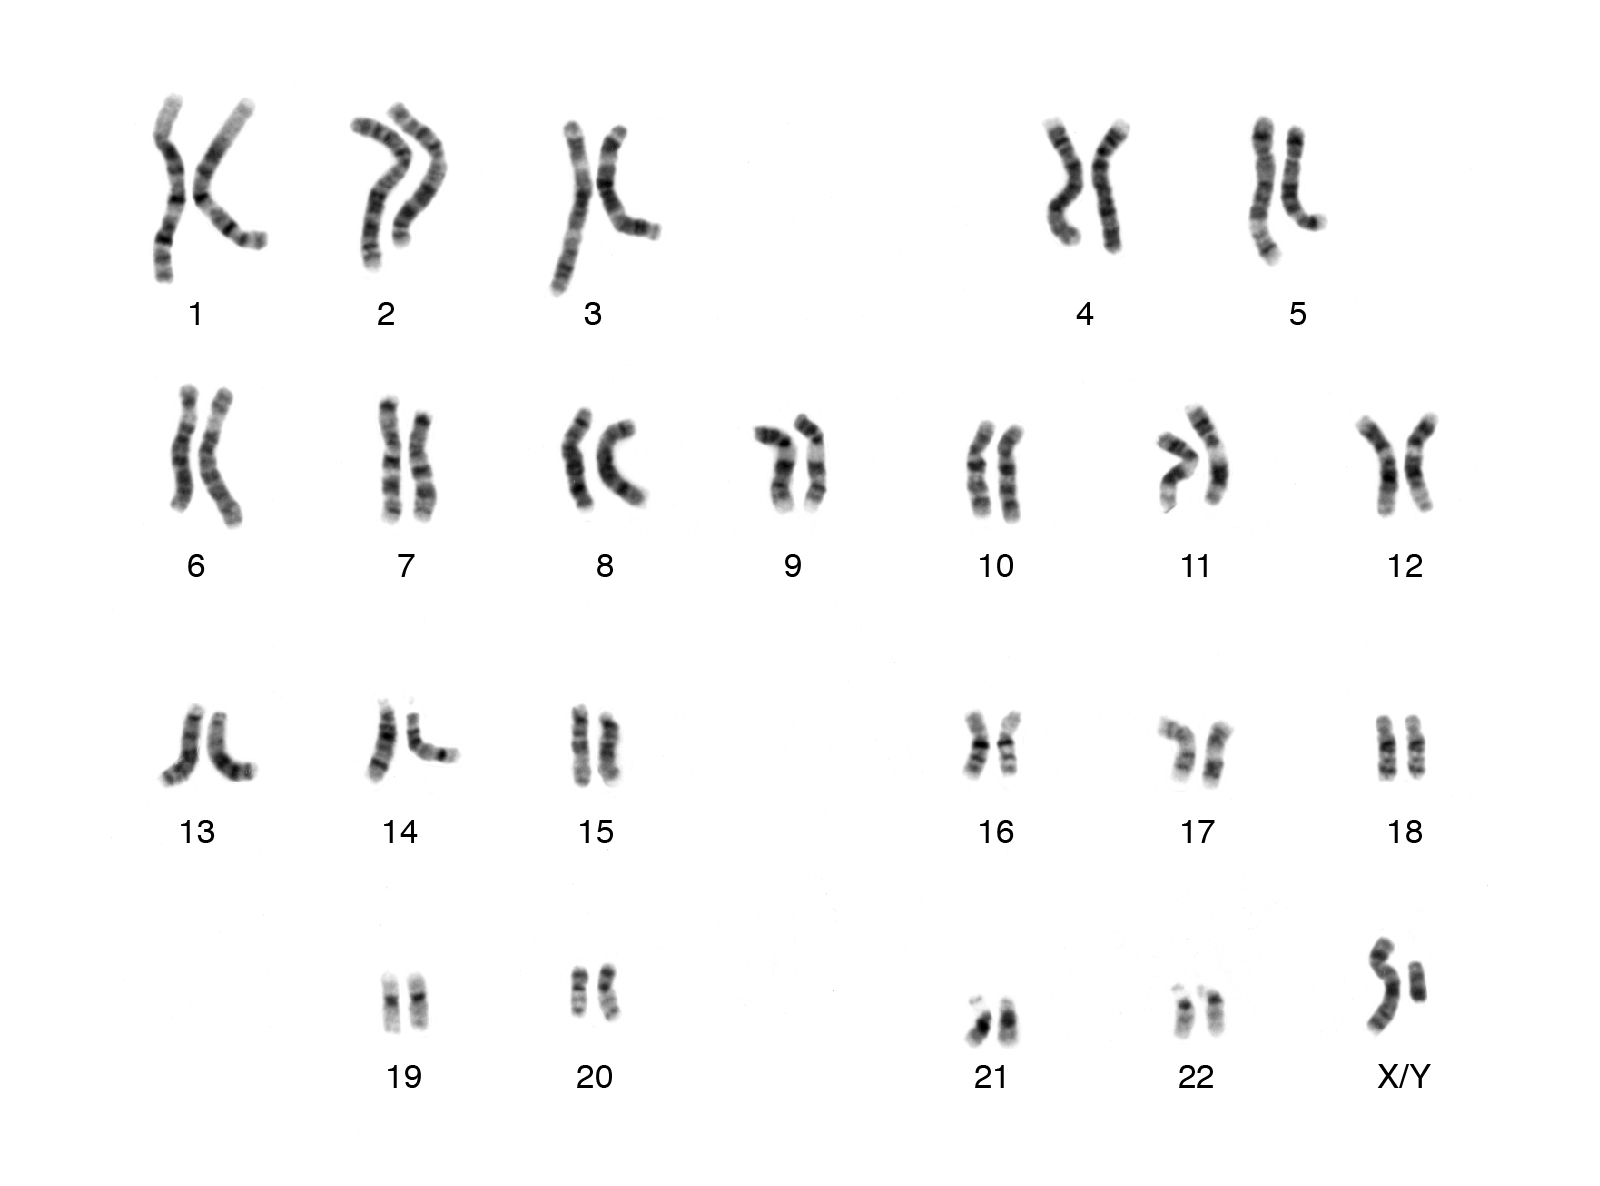
\includegraphics[width=0.8\textwidth,height=\textheight]{images/karyotype.jpg}

\vfill
\tiny

(Image taken from NHGRI)

\end{frame}

\hypertarget{central-dogma-of-molecular-biology}{%
\subsection{Central dogma of molecular
biology}\label{central-dogma-of-molecular-biology}}

\begin{frame}{Central dogma of molecular biology}
\protect\hypertarget{central-dogma-of-molecular-biology-1}{}

\centering

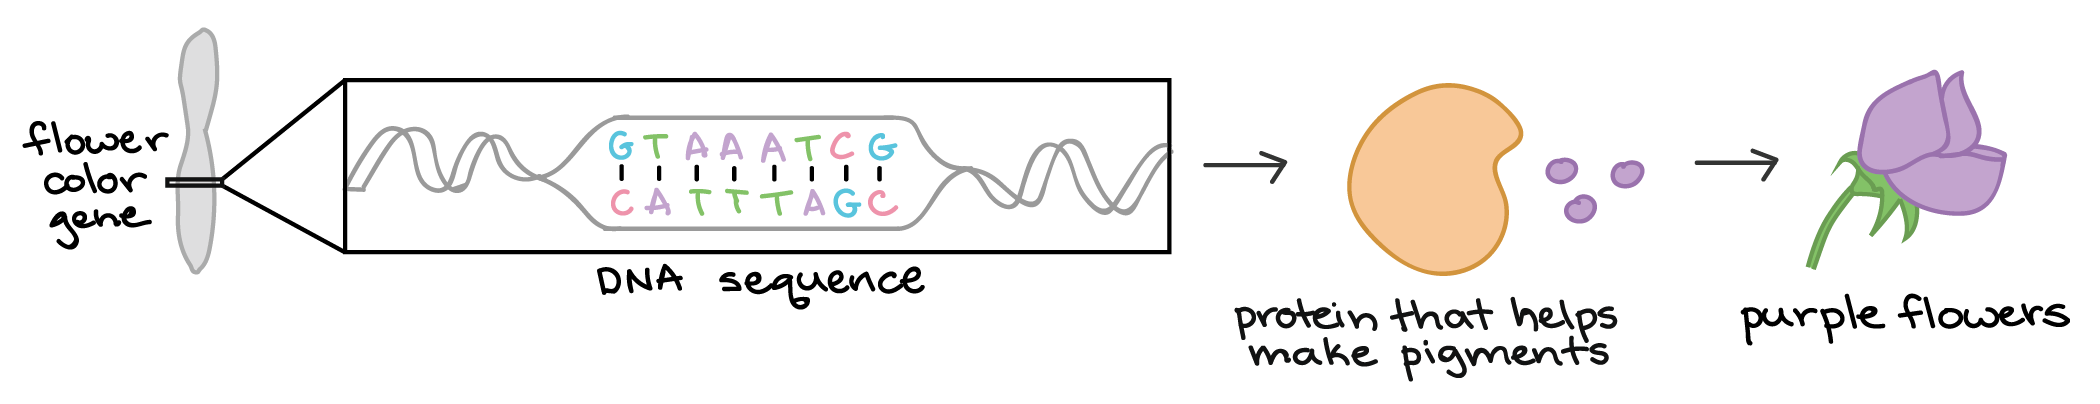
\includegraphics{images/geneToPheno.png}

\vfill
\tiny

(Image taken from Khan Academy)

\end{frame}

\begin{frame}{Central dogma of molecular biology}
\protect\hypertarget{central-dogma-of-molecular-biology-2}{}

\centering

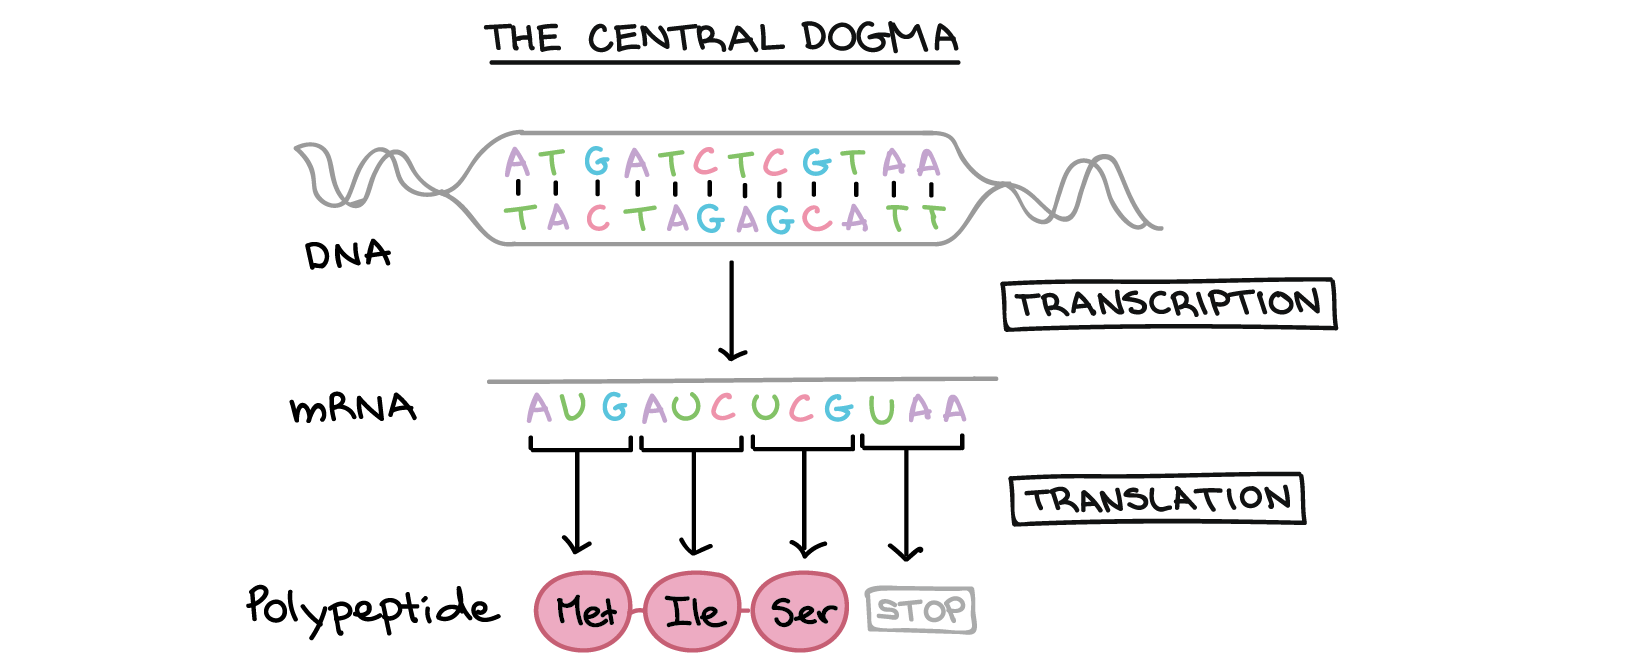
\includegraphics{images/centralDogma.png}

\vfill
\tiny

(Image taken from Khan Academy)

\end{frame}

\begin{frame}{Central dogma of molecular biology}
\protect\hypertarget{central-dogma-of-molecular-biology-3}{}

\centering

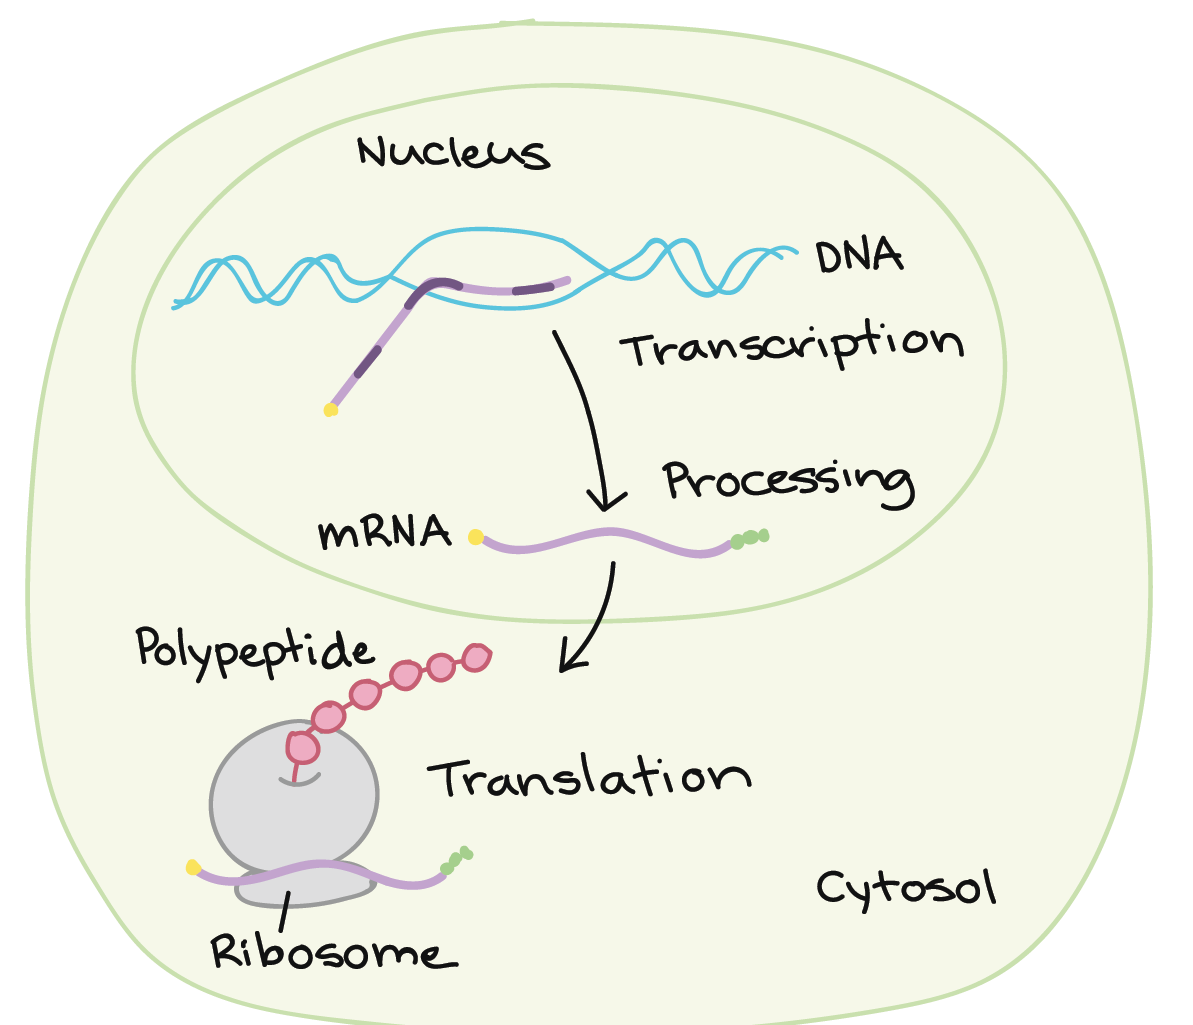
\includegraphics[width=0.5\textwidth,height=\textheight]{images/humanCell.png}

\vfill
\tiny

(Image taken from Khan Academy)

\end{frame}

\hypertarget{copy-number-variation-in-exome-sequencing}{%
\section{Copy number variation in exome
sequencing}\label{copy-number-variation-in-exome-sequencing}}

\hypertarget{background-and-motivation}{%
\subsection{Background and motivation}\label{background-and-motivation}}

\begin{frame}{What is a copy number variant?}
\protect\hypertarget{what-is-a-copy-number-variant}{}

\centering

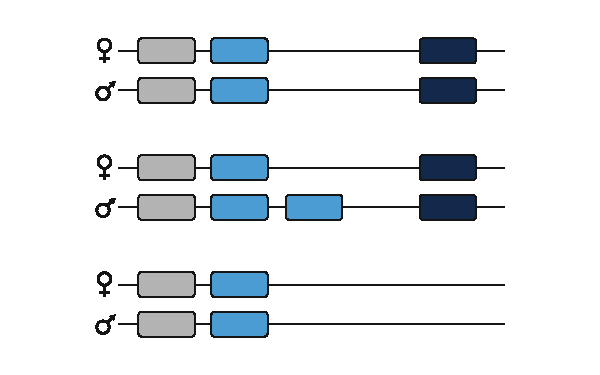
\includegraphics{images/cnvExamples.pdf}

\end{frame}

\begin{frame}{Motivation}
\protect\hypertarget{motivation}{}

\centering

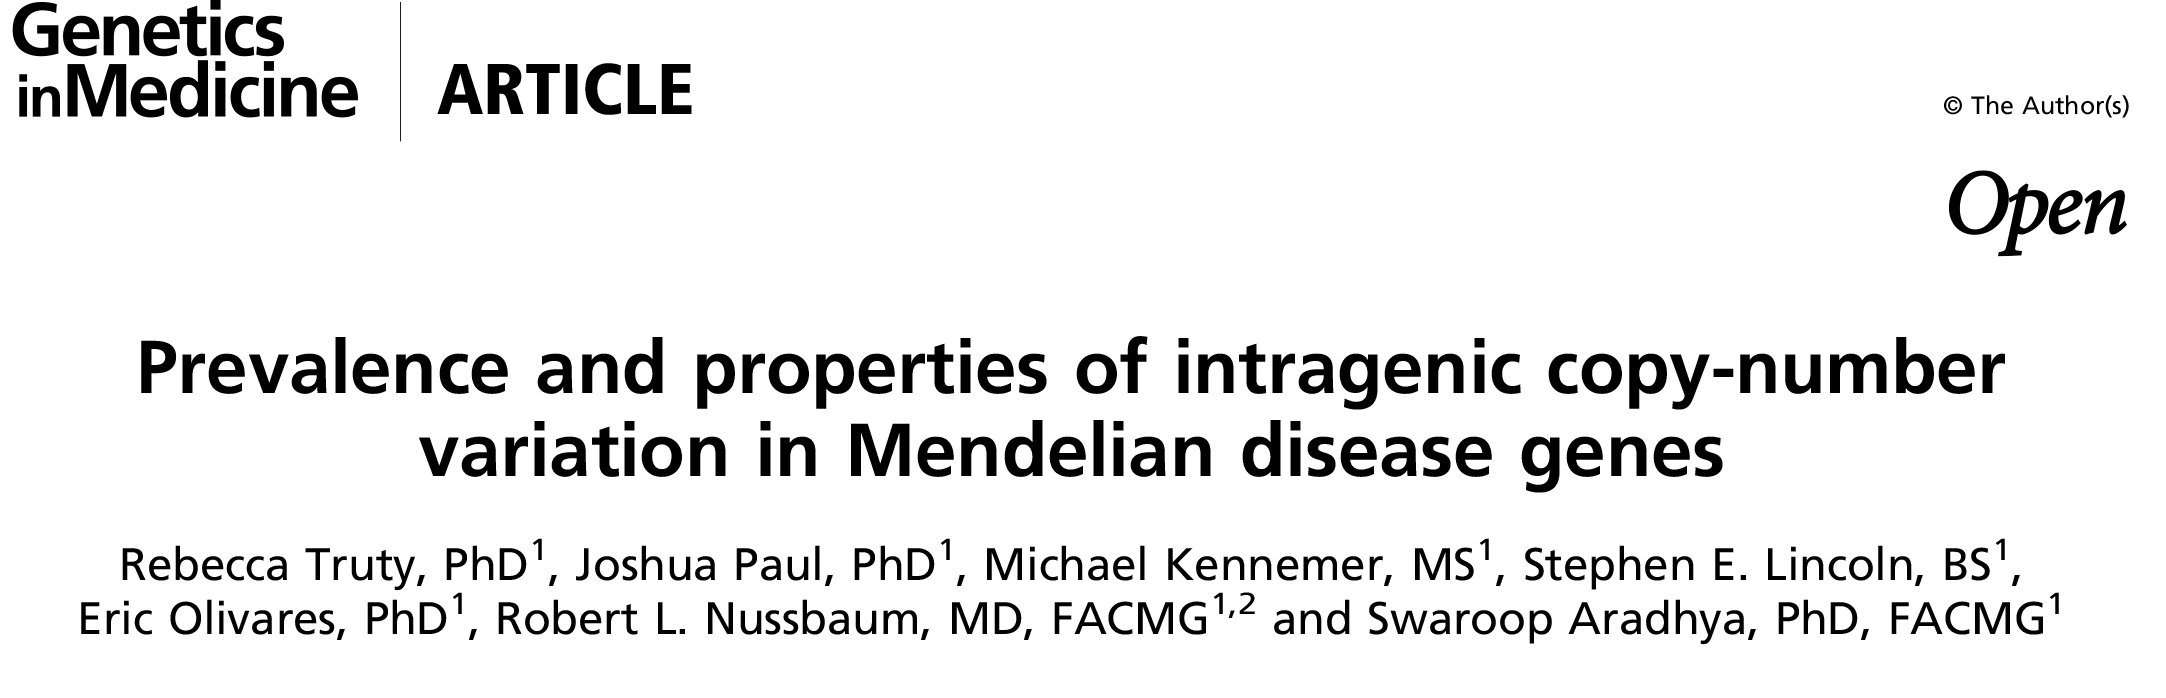
\includegraphics{images/truty.png}

\bigskip

\begin{quote}
Our analysis identified 2844 intragenic CNVs in 384 clinically tested
genes. CNVs were observed in 1.9\% of the entire cohort but in a
disproportionately high fraction (9.8\%) of individuals with a
clinically significant result.
\end{quote}

\end{frame}

\begin{frame}{Motivation}
\protect\hypertarget{motivation-1}{}

\centering

\begin{center}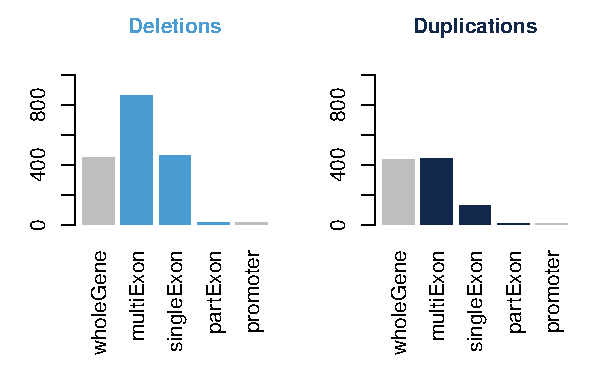
\includegraphics{defense_files/figure-beamer/truty-1} \end{center}

\end{frame}

\begin{frame}{The current state-of-the-art: ExomeDepth}
\protect\hypertarget{the-current-state-of-the-art-exomedepth}{}

\centering

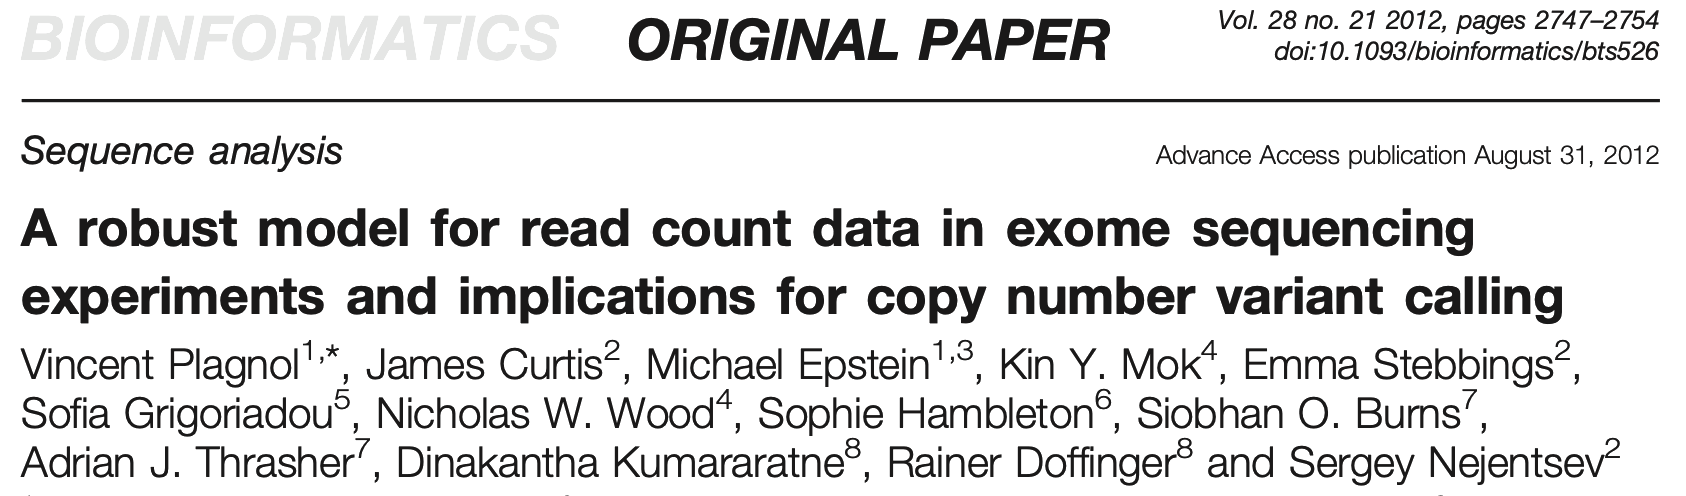
\includegraphics{images/exomeDepth.png} \raggedright

\begin{itemize}
\item
  ExomeDepth builds a comparative model based on the beta-binomial
  distribution
\item
  Begins by finding highly-correlated samples to build a control vector
\item
  Defaults to an expected CNV size of 50kb -- it does not perform well
  for small (exon level) variation
\end{itemize}

\end{frame}

\hypertarget{better-capturing-the-exome}{%
\subsection{Better capturing the
exome}\label{better-capturing-the-exome}}

\begin{frame}{Exome capture}
\protect\hypertarget{exome-capture}{}

\centering

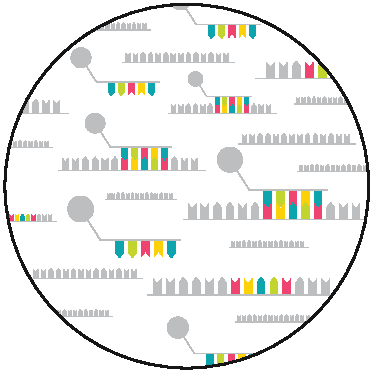
\includegraphics{images/captureBubble.pdf}

\end{frame}

\begin{frame}{Exon-to-exon capture variation}
\protect\hypertarget{exon-to-exon-capture-variation}{}

\begin{center}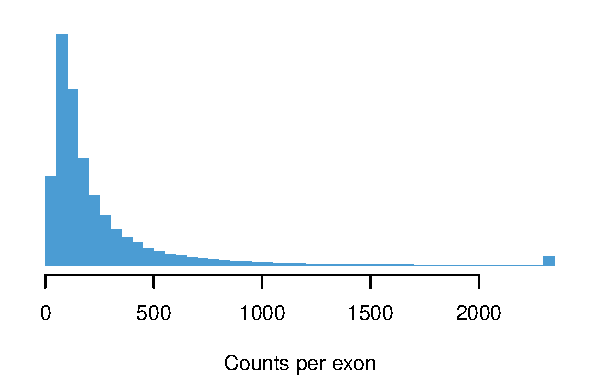
\includegraphics{defense_files/figure-beamer/exonCapVar-1} \end{center}

\end{frame}

\begin{frame}{Can we better capture exomes?}
\protect\hypertarget{can-we-better-capture-exomes}{}

\centering

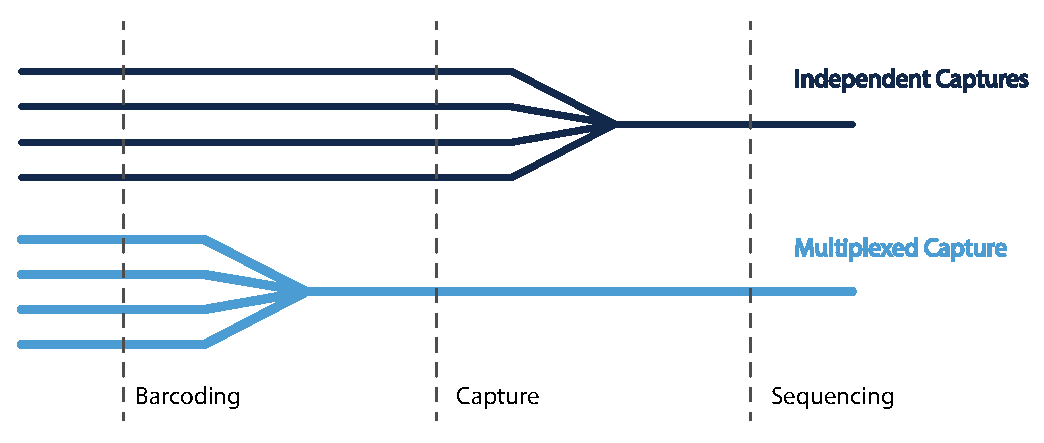
\includegraphics{images/multiCapture.pdf}

\end{frame}

\begin{frame}{Can we better capture exomes?}
\protect\hypertarget{can-we-better-capture-exomes-1}{}

\centering

\begin{tabular}{llrrrr}
\toprule
pool & capture & N & medExon & medTotal & rsdTotal\\
\midrule
IDT-IC$^\dagger$ & IDT & 16 & 143 & 55,149,058 & 22.4\\
IDT-MC & IDT & 16 & 93 & 29,772,684 & 64.2\\
IDT-RR & IDT & 16 & 272 & 79,079,629 & 22.9\\
NCGENES$^\dagger$ & Agilent & 112 & 93 & 24,451,245 & 27.6\\
Pool1 & Agilent & 16 & 56 & 13,265,614 & 18.5\\
\addlinespace
Pool2 & Agilent & 16 & 86 & 21,076,056 & 27.6\\
SMA1 & Agilent & 8 & 56 & 12,256,002 & 6.2\\
SMA2 & Agilent & 8 & 25 & 5,622,040 & 10.4\\
WGS & Agilent & 16 & 196 & 46,406,224 & 16.4\\
\bottomrule
\end{tabular}

\end{frame}

\begin{frame}{Can we better capture exomes?}
\protect\hypertarget{can-we-better-capture-exomes-2}{}

\begin{center}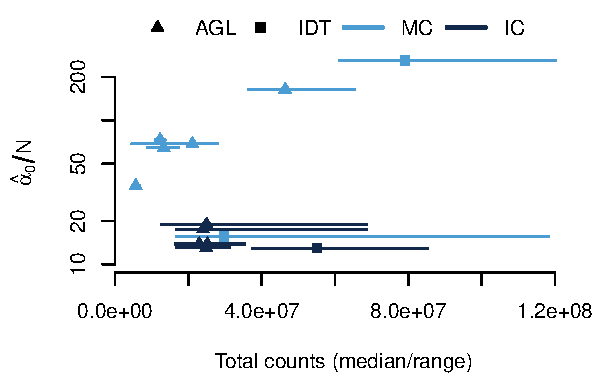
\includegraphics{defense_files/figure-beamer/a0plt-1} \end{center}

\end{frame}

\begin{frame}{Can we better capture exomes?}
\protect\hypertarget{can-we-better-capture-exomes-3}{}

\begin{center}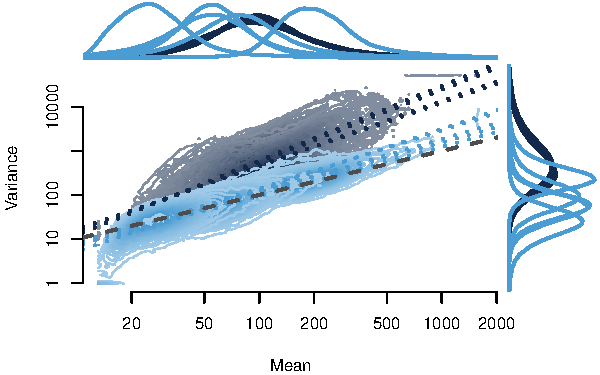
\includegraphics{defense_files/figure-beamer/aglMnVr-1} \end{center}

\end{frame}

\begin{frame}{Can we better capture exomes?}
\protect\hypertarget{can-we-better-capture-exomes-4}{}

\begin{center}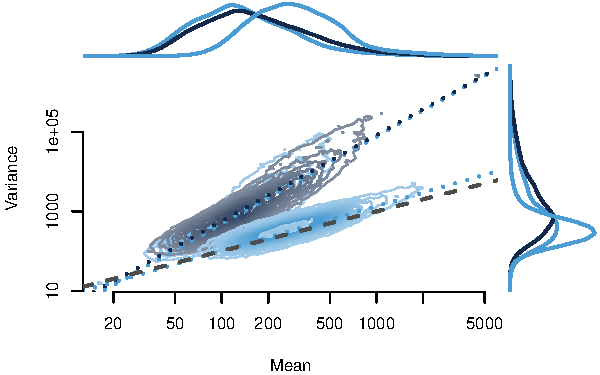
\includegraphics{defense_files/figure-beamer/idtMnVr-1} \end{center}

\end{frame}

\begin{frame}{Can we better capture exomes?}
\protect\hypertarget{can-we-better-capture-exomes-5}{}

\begin{center}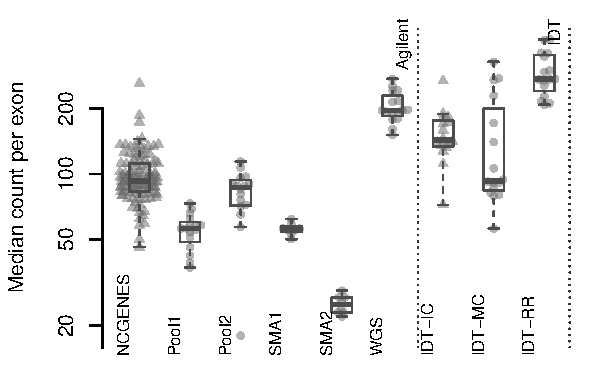
\includegraphics{defense_files/figure-beamer/medIntMolCount-1} \end{center}

\end{frame}

\begin{frame}{Can we better capture exomes?}
\protect\hypertarget{can-we-better-capture-exomes-6}{}

\begin{center}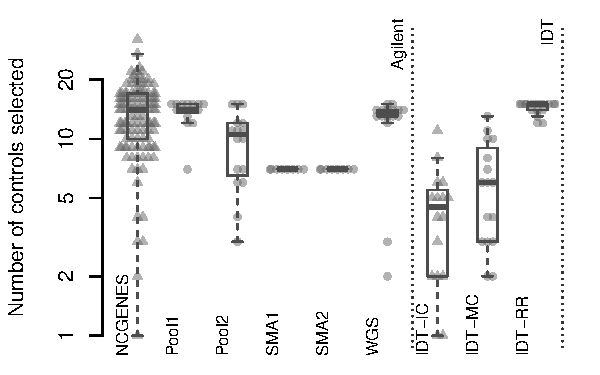
\includegraphics{defense_files/figure-beamer/nSelected-1} \end{center}

\end{frame}

\begin{frame}{Can we better capture exomes?}
\protect\hypertarget{can-we-better-capture-exomes-7}{}

\begin{center}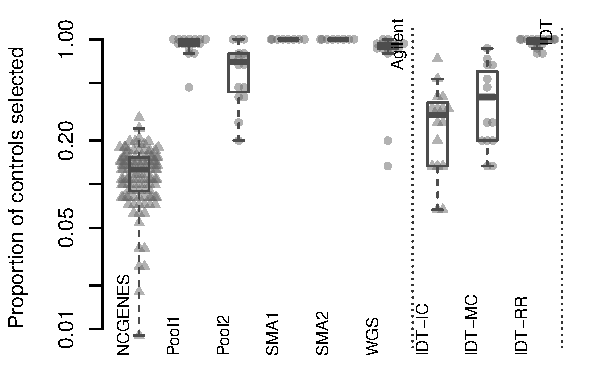
\includegraphics{defense_files/figure-beamer/propSelected-1} \end{center}

\end{frame}

\begin{frame}{Can we better capture exomes?}
\protect\hypertarget{can-we-better-capture-exomes-8}{}

\begin{center}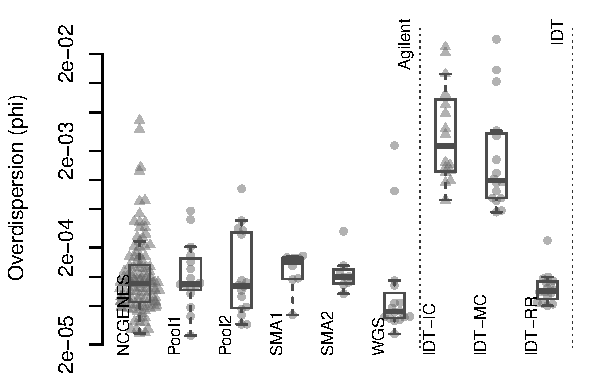
\includegraphics{defense_files/figure-beamer/overallPhi-1} \end{center}

\end{frame}

\begin{frame}{Can we better capture exomes?}
\protect\hypertarget{can-we-better-capture-exomes-9}{}

\bigskip

\centering\Huge\textcolor{uncnavy}{Yes!}

\bigskip
\raggedright\normalsize

\begin{block}{We recommend}

\begin{enumerate}
\item
  Multiplexing roughly 16 samples prior to exome capture
\item
  Checking for library balance prior to exome capture (from our limited
  data, we suggest RSD 30\%)
\end{enumerate}

\end{block}

\end{frame}

\hypertarget{novel-copy-number-variant-algorithm}{%
\subsection{Novel copy number variant
algorithm}\label{novel-copy-number-variant-algorithm}}

\begin{frame}{Can we better analyze exomes?}
\protect\hypertarget{can-we-better-analyze-exomes}{}

\begin{block}{mcCNV algorithm}

\medskip

\begin{enumerate}
\tightlist
\item
  Assumes multiplexed capture
\item
  Models observed counts using the negative binomial model
\item
  Uses a shrinkage estimator for the dispersion
\end{enumerate}

\medskip

\hfill 
\includegraphics[width=0.3\textwidth,height=\textheight]{images/mcCNV.png}

\end{block}

\end{frame}

\begin{frame}{Can we better analyze exomes?}
\protect\hypertarget{can-we-better-analyze-exomes-1}{}

\begin{center}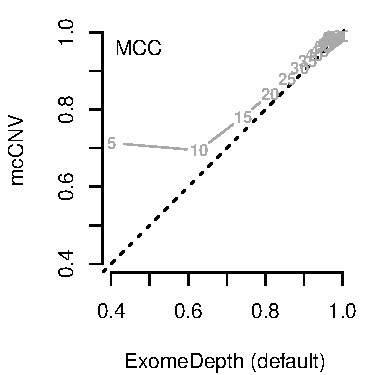
\includegraphics[width=0.49\linewidth]{defense_files/figure-beamer/simResMCC-1} 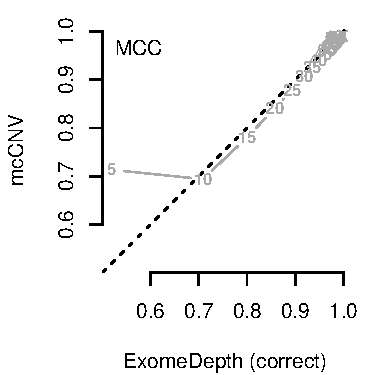
\includegraphics[width=0.49\linewidth]{defense_files/figure-beamer/simResMCC-2} \end{center}

\end{frame}

\begin{frame}{Can we better analyze exomes?}
\protect\hypertarget{can-we-better-analyze-exomes-2}{}

\begin{center}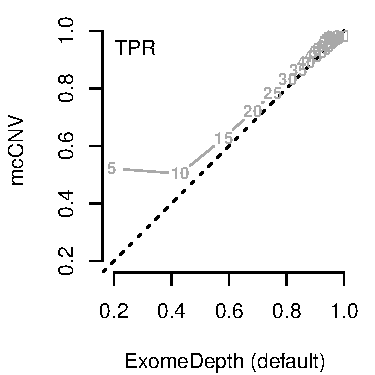
\includegraphics[width=0.49\linewidth]{defense_files/figure-beamer/simResTPR-1} 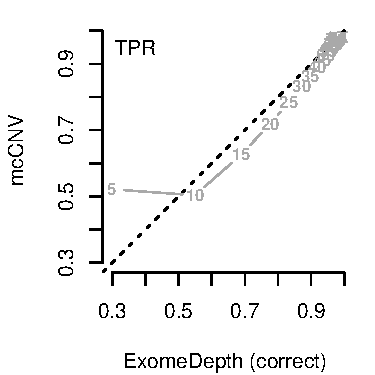
\includegraphics[width=0.49\linewidth]{defense_files/figure-beamer/simResTPR-2} \end{center}

\end{frame}

\begin{frame}{Can we better analyze exomes?}
\protect\hypertarget{can-we-better-analyze-exomes-3}{}

\begin{center}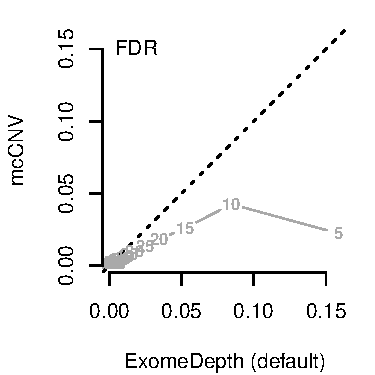
\includegraphics[width=0.49\linewidth]{defense_files/figure-beamer/simResFDR-1} 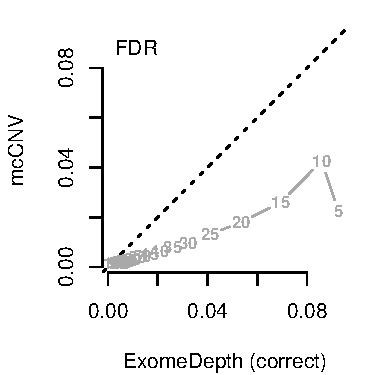
\includegraphics[width=0.49\linewidth]{defense_files/figure-beamer/simResFDR-2} \end{center}

\end{frame}

\begin{frame}{Can we better analyze exomes?}
\protect\hypertarget{can-we-better-analyze-exomes-4}{}

\centering

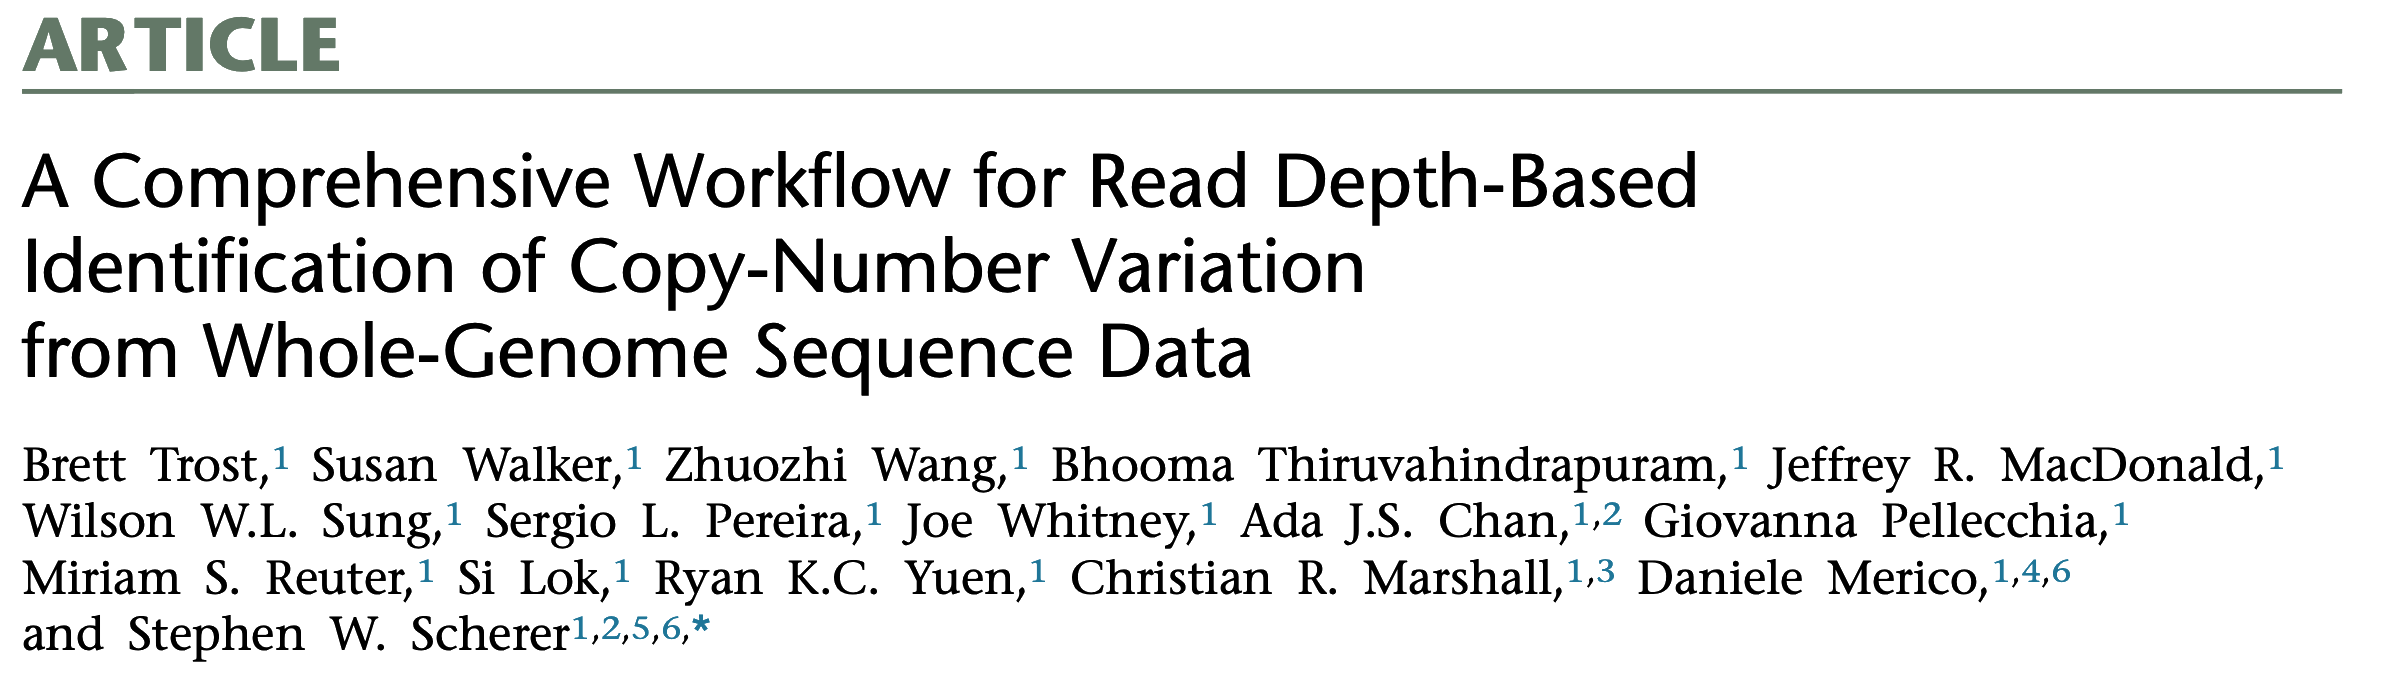
\includegraphics{images/trost.png} \raggedright

\begin{itemize}
\item
  Combines calls from two algorithms: ERDS and CNVnator
\item
  Excludes repetitive and low-complexity regions (RCLRs)
\item
  Followed their recommendations, and removed all exons overlapping
  their defined RLCRs
\end{itemize}

\end{frame}

\begin{frame}{Can we better analyze exomes?}
\protect\hypertarget{can-we-better-analyze-exomes-5}{}

\scriptsize

\begin{table}[H]
\centering
\begin{tabular}{lrrrrrrrrr}
\toprule
\multicolumn{1}{c}{ } & \multicolumn{3}{c}{Total} & \multicolumn{3}{c}{Duplications} & \multicolumn{3}{c}{Deletions} \\
\cmidrule(l{3pt}r{3pt}){2-4} \cmidrule(l{3pt}r{3pt}){5-7} \cmidrule(l{3pt}r{3pt}){8-10}
subject & MC & ED & WG & MC & ED & WG & MC & ED & WG\\
\midrule
NCG\_00012 & 90 & 106 & 143 & 61 & 73 & 121 & 29 & 33 & 22\\
NCG\_00237 & 82 & 101 & 165 & 50 & 64 & 129 & 32 & 37 & 36\\
NCG\_00525 & 68 & 74 & 151 & 30 & 33 & 110 & 38 & 41 & 41\\
NCG\_00593 & 45 & 58 & 142 & 22 & 28 & 81 & 23 & 30 & 61\\
NCG\_00676 & 66 & 78 & 112 & 38 & 46 & 92 & 28 & 32 & 20\\
NCG\_00790 & 5,156 & 2,204 & 121 & 19 & 37 & 92 & 5,137 & 2,167 & 29\\
NCG\_00819 & 68 & 76 & 134 & 30 & 41 & 100 & 38 & 35 & 34\\
NCG\_00840 & 78 & 92 & 157 & 44 & 52 & 115 & 34 & 40 & 42\\
NCG\_00851 & 1,151 & 859 & 141 & 28 & 51 & 102 & 1,123 & 808 & 39\\
NCG\_00857 & 59 & 75 & 119 & 10 & 15 & 81 & 49 & 60 & 38\\
NCG\_00976 & 46 & 58 & 114 & 25 & 37 & 93 & 21 & 21 & 21\\
NCG\_01023 & 59 & 95 & 143 & 32 & 60 & 113 & 27 & 35 & 30\\
NCG\_01043 & 73 & 94 & 128 & 40 & 64 & 105 & 33 & 30 & 23\\
NCG\_01076 & 36 & 57 & 105 & 7 & 22 & 78 & 29 & 35 & 27\\
NCG\_01077 & 135 & 157 & 230 & 103 & 121 & 184 & 32 & 36 & 46\\
NCG\_01117 & 95 & 101 & 154 & 72 & 78 & 129 & 23 & 23 & 25\\
\bottomrule
\end{tabular}
\end{table}

\end{frame}

\begin{frame}{Can we better analyze exomes?}
\protect\hypertarget{can-we-better-analyze-exomes-6}{}

\scriptsize

\begin{table}[H]
\centering
\begin{tabular}{>{}lllrrrr}
\toprule
 &  &  & MCC & TPR & FDR & PPV\\
\midrule
\cellcolor{uncgray}{} &  & MC & 0.185 & 0.335 & 0.897 & 0.1030\\

\cellcolor{uncgray}{} & \multirow{-2}{*}{\raggedright\arraybackslash Total} & ED & 0.263 & 0.363 & 0.809 & 0.1910\\

\cellcolor{uncgray}{} & \cellcolor{gray85}{} & \cellcolor{gray85}{MC} & \cellcolor{gray85}{0.487} & \cellcolor{gray85}{0.345} & \cellcolor{gray85}{0.311} & \cellcolor{gray85}{0.6890}\\

\cellcolor{uncgray}{\multirow{-4}{*}{\raggedright\arraybackslash ALL}} & \cellcolor{gray85}{\multirow{-2}{*}{\raggedright\arraybackslash Sub}} & \cellcolor{gray85}{ED} & \cellcolor{gray85}{0.482} & \cellcolor{gray85}{0.378} & \cellcolor{gray85}{0.383} & \cellcolor{gray85}{0.6170}\\
\cmidrule{1-7}
\cellcolor{uncgray}{} &  & MC & 0.396 & 0.236 & 0.334 & 0.6660\\

\cellcolor{uncgray}{} & \multirow{-2}{*}{\raggedright\arraybackslash Total} & ED & 0.347 & 0.240 & 0.496 & 0.5040\\

\cellcolor{uncgray}{} & \cellcolor{gray85}{} & \cellcolor{gray85}{MC} & \cellcolor{gray85}{0.404} & \cellcolor{gray85}{0.246} & \cellcolor{gray85}{0.333} & \cellcolor{gray85}{0.6670}\\

\cellcolor{uncgray}{\multirow{-4}{*}{\raggedright\arraybackslash DUP}} & \cellcolor{gray85}{\multirow{-2}{*}{\raggedright\arraybackslash Sub}} & \cellcolor{gray85}{ED} & \cellcolor{gray85}{0.384} & \cellcolor{gray85}{0.266} & \cellcolor{gray85}{0.446} & \cellcolor{gray85}{0.5540}\\
\cmidrule{1-7}
\cellcolor{uncgray}{} &  & MC & 0.180 & 0.639 & 0.949 & 0.0509\\

\cellcolor{uncgray}{} & \multirow{-2}{*}{\raggedright\arraybackslash Total} & ED & 0.219 & 0.558 & 0.914 & 0.0861\\

\cellcolor{uncgray}{} & \cellcolor{gray85}{} & \cellcolor{gray85}{MC} & \cellcolor{gray85}{0.683} & \cellcolor{gray85}{0.661} & \cellcolor{gray85}{0.294} & \cellcolor{gray85}{0.7060}\\

\cellcolor{uncgray}{\multirow{-4}{*}{\raggedright\arraybackslash DEL}} & \cellcolor{gray85}{\multirow{-2}{*}{\raggedright\arraybackslash Sub}} & \cellcolor{gray85}{ED} & \cellcolor{gray85}{0.541} & \cellcolor{gray85}{0.554} & \cellcolor{gray85}{0.471} & \cellcolor{gray85}{0.5290}\\
\bottomrule
\end{tabular}
\end{table}

\end{frame}

\begin{frame}{Can we better analyze exomes?}
\protect\hypertarget{can-we-better-analyze-exomes-7}{}

\begin{center}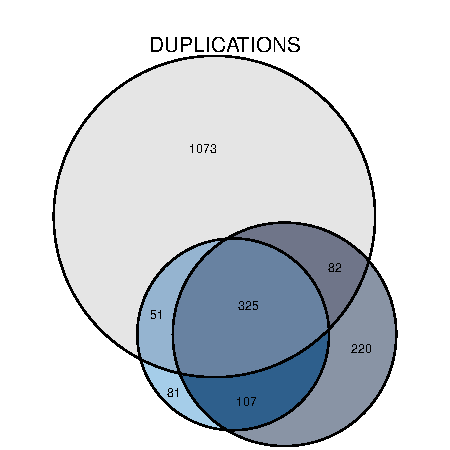
\includegraphics[width=0.49\linewidth]{defense_files/figure-beamer/vennSub-1} 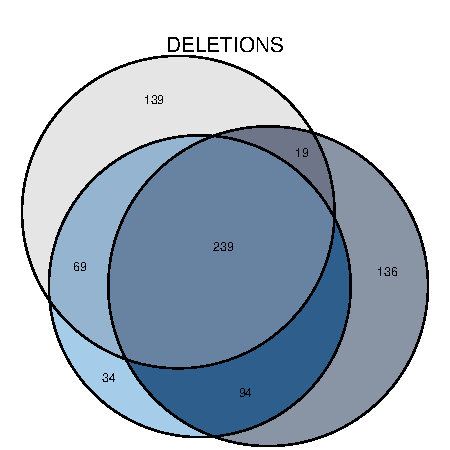
\includegraphics[width=0.49\linewidth]{defense_files/figure-beamer/vennSub-2} \end{center}

\begin{center}
\includegraphics{defense_files/figure-beamer/vennLgnd-1} \end{center}

\end{frame}

\begin{frame}{Can we better analyze exomes?}
\protect\hypertarget{can-we-better-analyze-exomes-8}{}

\bigskip

\centering\Huge\textcolor{uncnavy}{Possibly...}

\bigskip
\raggedright\normalsize

\begin{itemize}
\item
  Found comparable performance overall to ExomeDepth
\item
  However! We do not require prior information
\end{itemize}

\hfill 
\includegraphics[width=0.3\textwidth,height=\textheight]{images/mcCNV.png}

\end{frame}

\hypertarget{detecting-fetal-variation-from-cell-free-dna}{%
\section{Detecting fetal variation from cell-free
DNA}\label{detecting-fetal-variation-from-cell-free-dna}}

\hypertarget{background}{%
\subsection{Background}\label{background}}

\begin{frame}{Cell-free DNA used for fetal genetic testing}
\protect\hypertarget{cell-free-dna-used-for-fetal-genetic-testing}{}

\centering 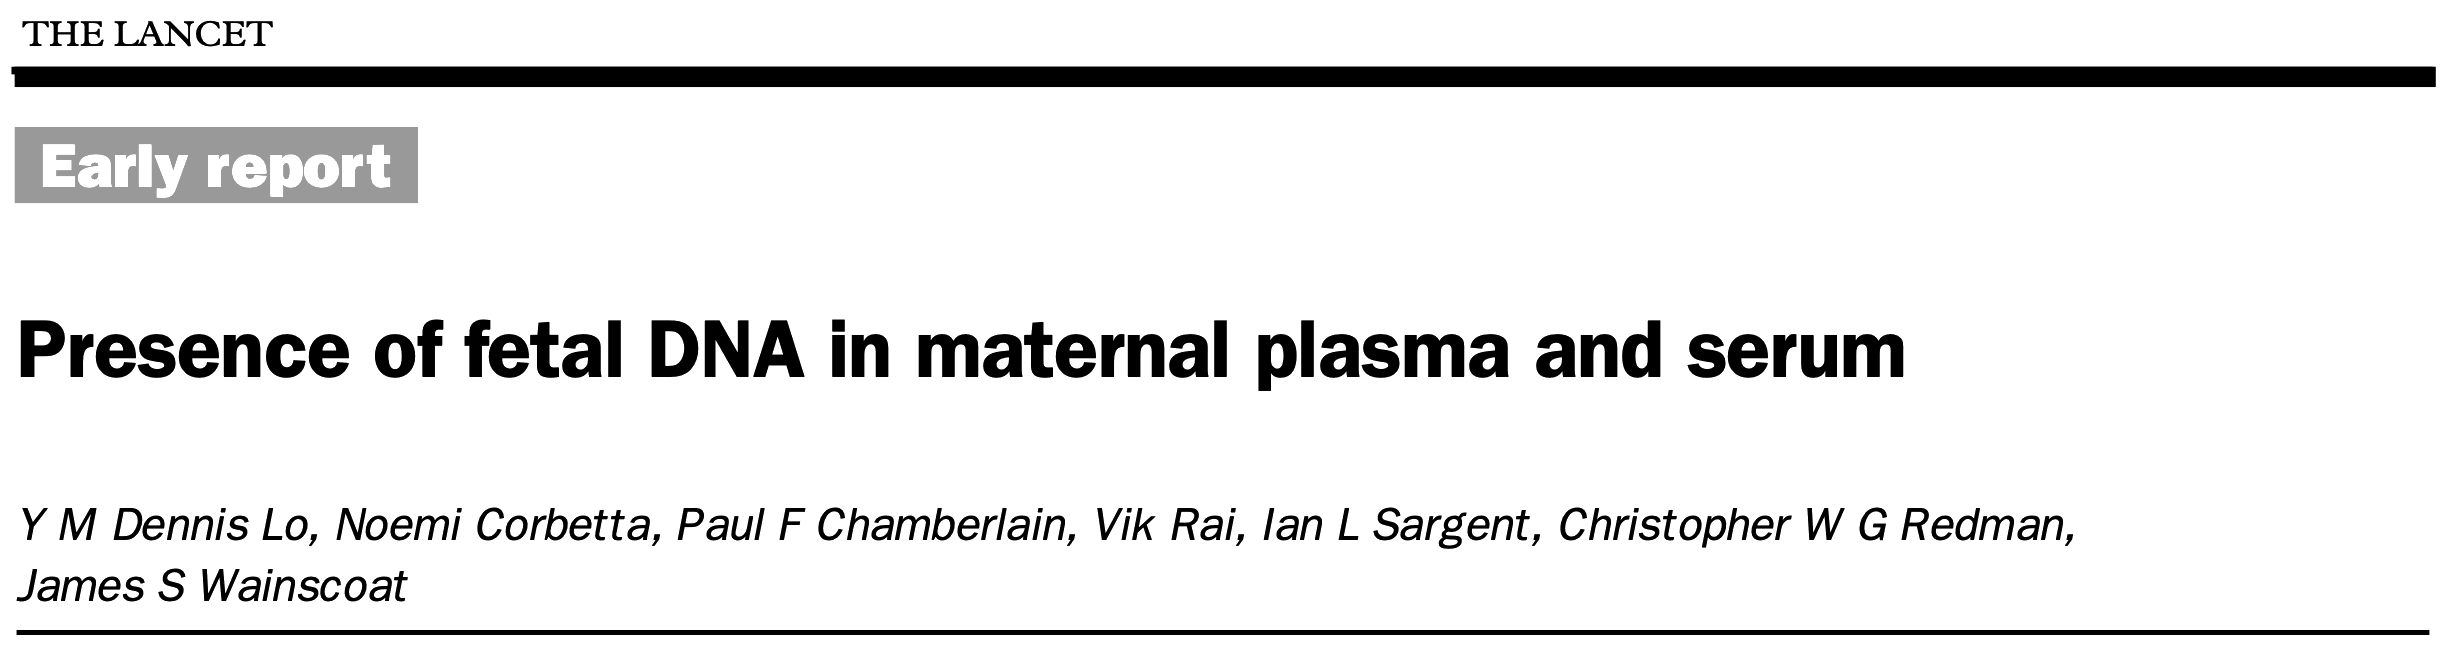
\includegraphics{images/lo.png}

\raggedright

\begin{block}{Noninvasive testing can now detect:}

\begin{itemize}
\item
  aneuploidy and large chromosomal deletions (\textgreater5Mb)
\item
  autosomal dominant single-gene disorders
\item
  autosomal recessive single-gene disorders using relative haplotype
  dosing (RHDO)
\end{itemize}

\end{block}

\end{frame}

\begin{frame}{Motivation}
\protect\hypertarget{motivation-2}{}

\centering

\textbf{\emph{No one has demonstrated accurate fetal genotyping from
cell-free DNA without additional parental sequencing}}

\bigskip\bigskip\raggedright

Fetal genotyping using only cell-free DNA would

\begin{enumerate}
\item
  enable population-level screening for Mendelian disorders, allowing
  immediate neonatal management;
\item
  provide more targets for developing \emph{in utero} therapies.
\end{enumerate}

\end{frame}

\begin{frame}{The two estimation problems}
\protect\hypertarget{the-two-estimation-problems}{}

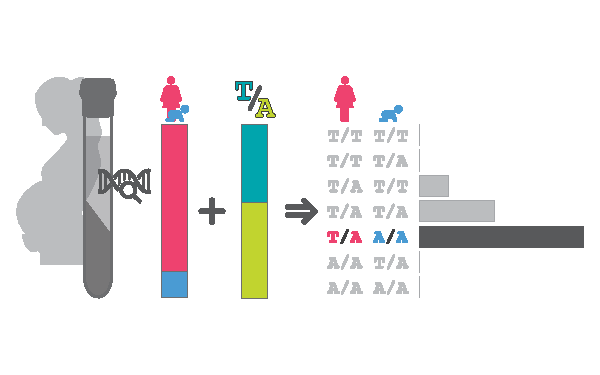
\includegraphics{images/cellFreeDiagram.pdf}

\end{frame}

\begin{frame}{Estimating fetal fraction}
\protect\hypertarget{estimating-fetal-fraction}{}

Represent maternal and fetal genotype pairs with capital and lowercase
letters, where `A' and `B' represent the major and minor alleles
(e.g.~`AAab' represents the fetus uniquely heterozygous for the minor
allele). Define the fetal fraction and PMAR as the random variables
\(F\) and \(M\).

\begin{align}
\text{E}[M \rvert G = \text{AAab}, F = f] &= \frac{f}{2} \\
\text{E}[M \rvert G = \text{ABaa}, F = f] &= \frac{1 - f}{2} \\
\text{E}[M \rvert G = \text{ABab}, F = f] &= \frac{1}{2} \\
\text{E}[M \rvert G = \text{ABbb}, F = f] &= \frac{1 + f}{2} \\
\text{E}[M \rvert G = \text{BBab}, F = f] &= 1 - \frac{f}{2} 
\end{align}

\end{frame}

\begin{frame}{Estimating fetal fraction}
\protect\hypertarget{estimating-fetal-fraction-1}{}

\begin{center}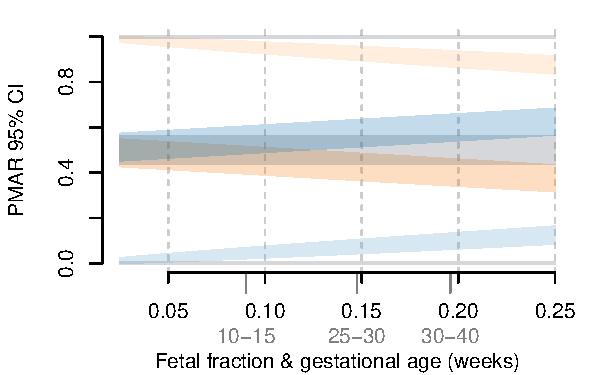
\includegraphics{defense_files/figure-beamer/expMaf250-1} \end{center}

\centering 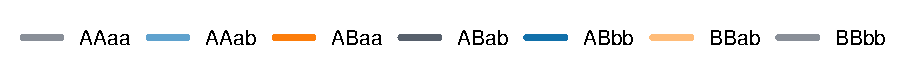
\includegraphics{defense_files/figure-beamer/genoLgnd-1.pdf}

\end{frame}

\hypertarget{novel-maternal-fetal-genotyping-algorithm}{%
\subsection{Novel maternal-fetal genotyping
algorithm}\label{novel-maternal-fetal-genotyping-algorithm}}

\begin{frame}{Novel maternal-fetal genotyping algorithm}
\protect\hypertarget{novel-maternal-fetal-genotyping-algorithm-1}{}

\begin{itemize}
\item
  Perform empirical Bayes EM routine to identify unique fetal
  heterozygosity
\item
  Estimate fetal fraction as the median across all sites with fetal
  heterozygosity
\item
  Estimate maternal-fetal genotypes as the maximal-likelihood given the
  fetal fraction estimate
\end{itemize}

\end{frame}

\hypertarget{shortcomings-of-noninvasive-exome-sequencing}{%
\subsection{Shortcomings of noninvasive exome
sequencing}\label{shortcomings-of-noninvasive-exome-sequencing}}

\begin{frame}{Applying genotyping algorithm to cell-free exome
sequencing}
\protect\hypertarget{applying-genotyping-algorithm-to-cell-free-exome-sequencing}{}

\scriptsize

\begin{table}
\centering
\begin{tabular}[t]{ll>{\raggedright\arraybackslash}p{8em}>{\raggedright\arraybackslash}p{8em}rrrr}
\toprule
  & GA & Clinical findings & Genetic diagnosis & FF & Dep & \%Dup & \%Filt\\
\midrule
1 & 32w2d & 5 prior pregnancies affected with X-linked recessive Menke's syndrome & Menke's syndrome; del. ATP7A exon 1 & 0.117 & 241 & 42.80 & 21.96\\
2 & 24w5d & Fetal sonogram at 21w5d showed femoral bowing with shortened length (\textless3\% for GA) bilaterally & Osteogenesis imperfecta type VIII; P3H1 c.1120G\textgreater T (rs140468248) & 0.122 & 152 & 33.32 & 22.09\\
3 & 34w0d & Fetal sonogram at 19w0d showed bilateral club foot with bilateral upper limb arthrogryposis & None, to date, despite exome and genome sequencing of newborn & 0.169 & 330 & 53.67 & 32.65\\
\bottomrule
\end{tabular}
\end{table}

\end{frame}

\begin{frame}{Applying genotyping algorithm to cell-free exome
sequencing}
\protect\hypertarget{applying-genotyping-algorithm-to-cell-free-exome-sequencing-1}{}

\begin{center}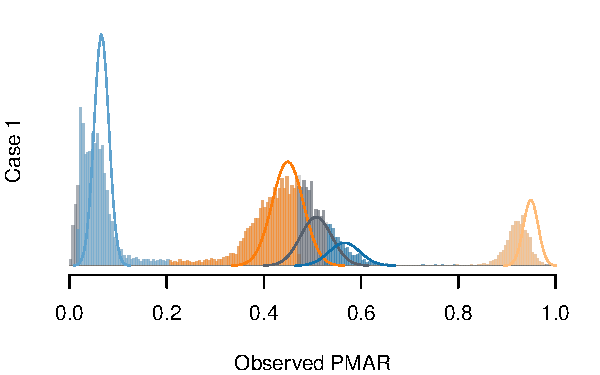
\includegraphics{defense_files/figure-beamer/alleleDepCase1-1} \end{center}

\centering 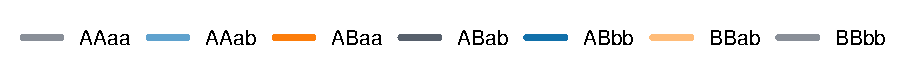
\includegraphics{defense_files/figure-beamer/genoLgnd-1.pdf}

\end{frame}

\begin{frame}{Applying genotyping algorithm to cell-free exome
sequencing}
\protect\hypertarget{applying-genotyping-algorithm-to-cell-free-exome-sequencing-2}{}

\begin{center}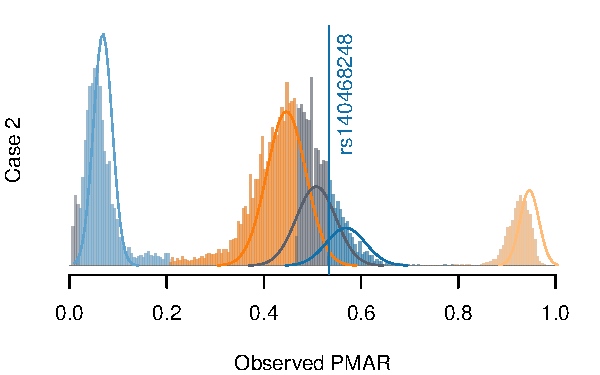
\includegraphics{defense_files/figure-beamer/alleleDepCase2-1} \end{center}

\centering 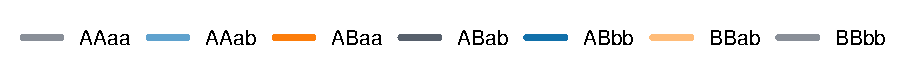
\includegraphics{defense_files/figure-beamer/genoLgnd-1.pdf}

\end{frame}

\begin{frame}{Applying genotyping algorithm to cell-free exome
sequencing}
\protect\hypertarget{applying-genotyping-algorithm-to-cell-free-exome-sequencing-3}{}

\begin{center}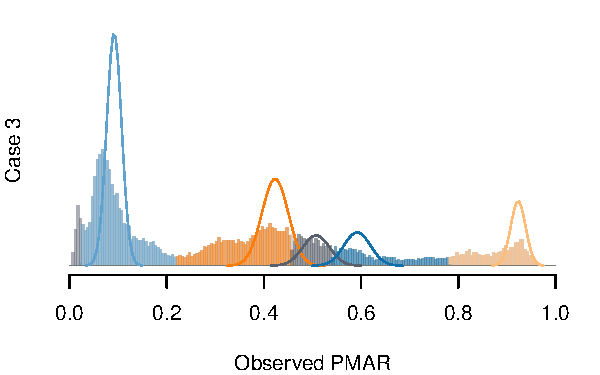
\includegraphics{defense_files/figure-beamer/alleleDepCase3-1} \end{center}

\centering 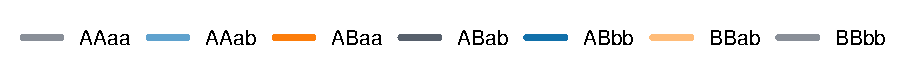
\includegraphics{defense_files/figure-beamer/genoLgnd-1.pdf}

\end{frame}

\begin{frame}{Applying genotyping algorithm to cell-free exome
sequencing}
\protect\hypertarget{applying-genotyping-algorithm-to-cell-free-exome-sequencing-4}{}

\begin{itemize}
\item
  In Case 3, we also have individual exome sequencing for the mother,
  father, and fetus
\item
  Overall, we found a 50.91\% genotyping accuracy
\end{itemize}

\bigskip

\begin{table}[H]
\centering
\begin{tabular}{llrrr}
\toprule
\multicolumn{2}{c}{ } & \multicolumn{3}{c}{Cell-free} \\
\cmidrule(l{3pt}r{3pt}){3-5}
  &   & 0/0 & 0/1 & 1/1\\
\midrule
 & 0/0 & 1,063 & 1,857 & 9\\
\cmidrule{2-5}
 & 0/1 & 3,598 & 7,079 & 1,454\\
\cmidrule{2-5}
\multirow{-3}{*}{\raggedright\arraybackslash Fetal} & 1/1 & 76 & 2,197 & 1,391\\
\bottomrule
\end{tabular}
\end{table}

\end{frame}

\begin{frame}{Explaining the poor performance}
\protect\hypertarget{explaining-the-poor-performance}{}

\begin{center}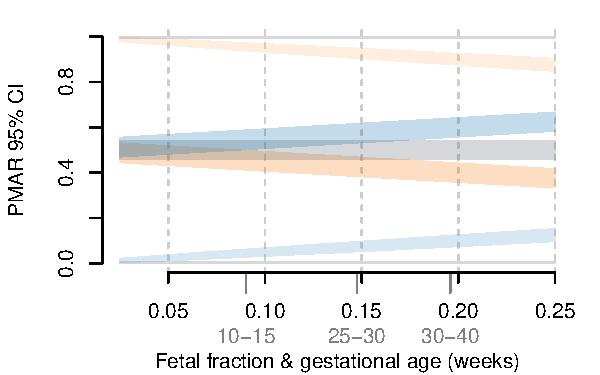
\includegraphics{defense_files/figure-beamer/binCI-1} \end{center}

\end{frame}

\begin{frame}{Explaining the poor performance}
\protect\hypertarget{explaining-the-poor-performance-1}{}

\begin{center}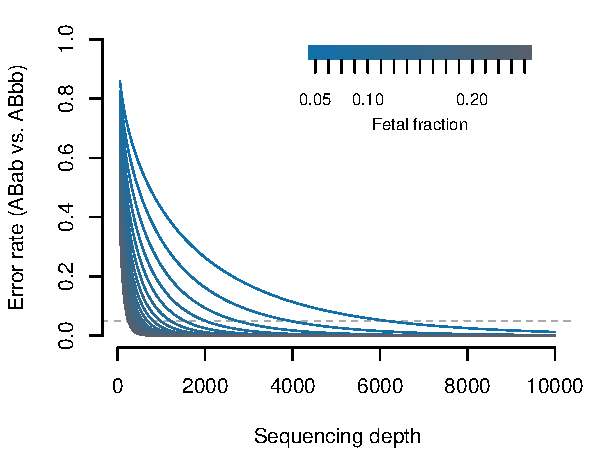
\includegraphics{defense_files/figure-beamer/binWeitz-1} \end{center}

\end{frame}

\begin{frame}{Does fragment length matter?}
\protect\hypertarget{does-fragment-length-matter}{}

\centering 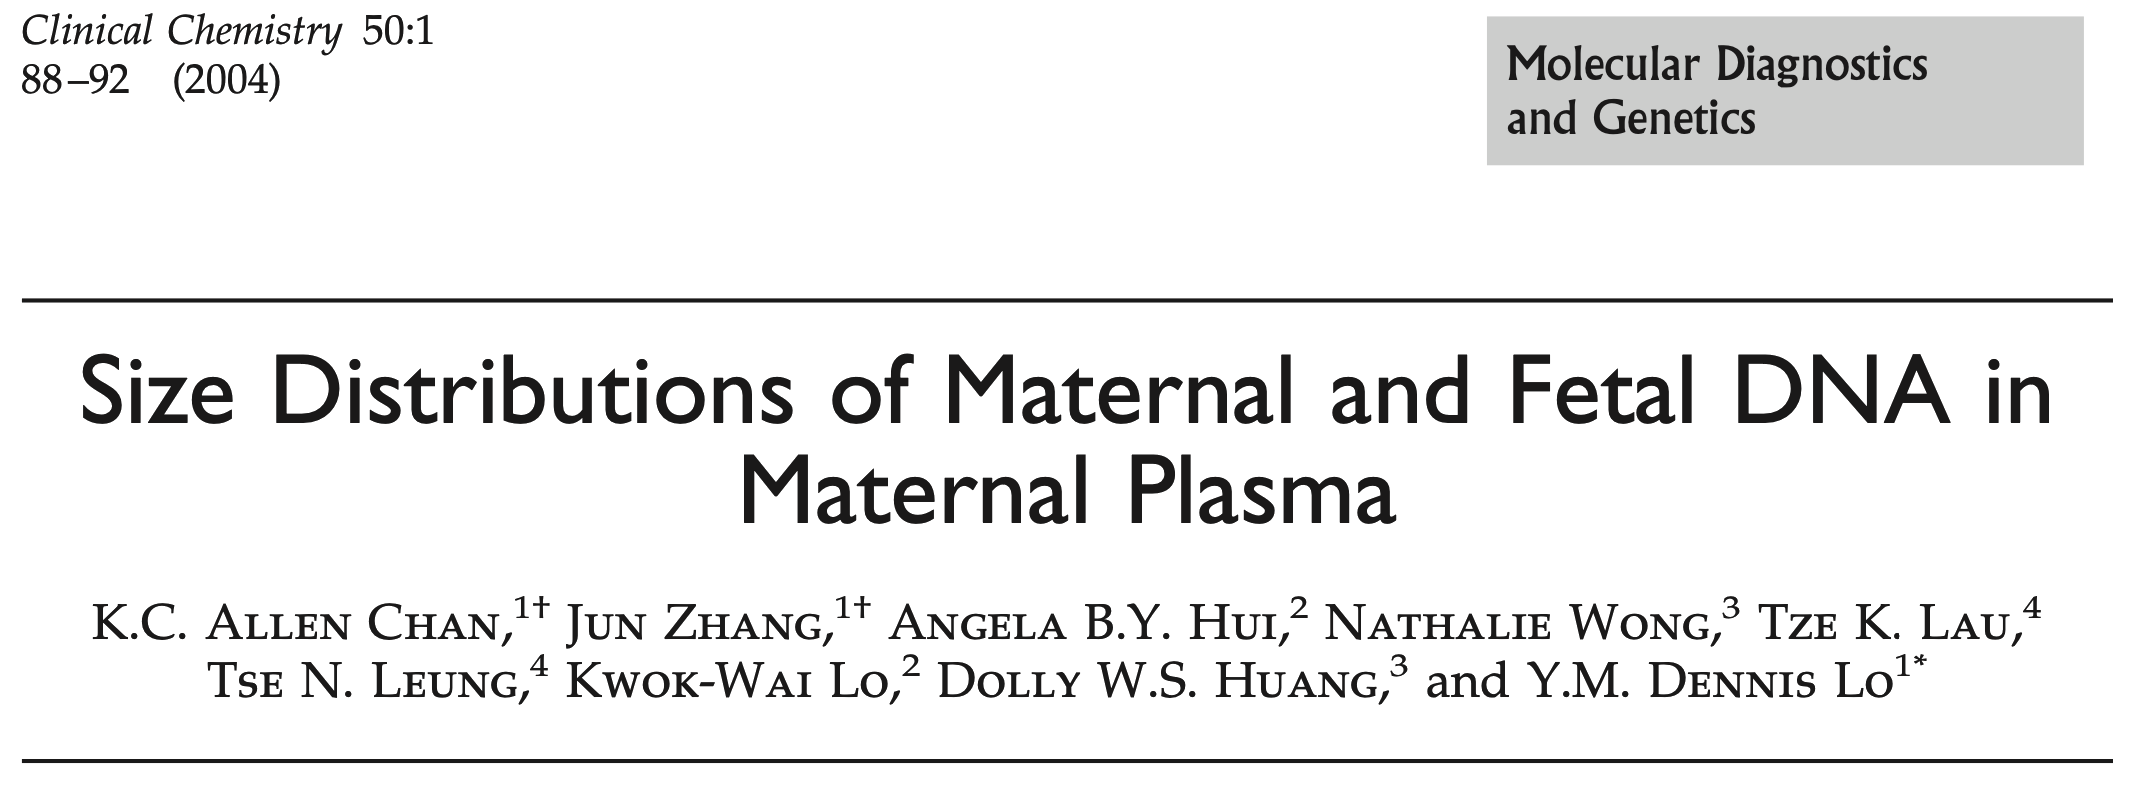
\includegraphics{images/chan.png}

\bigskip

\centering 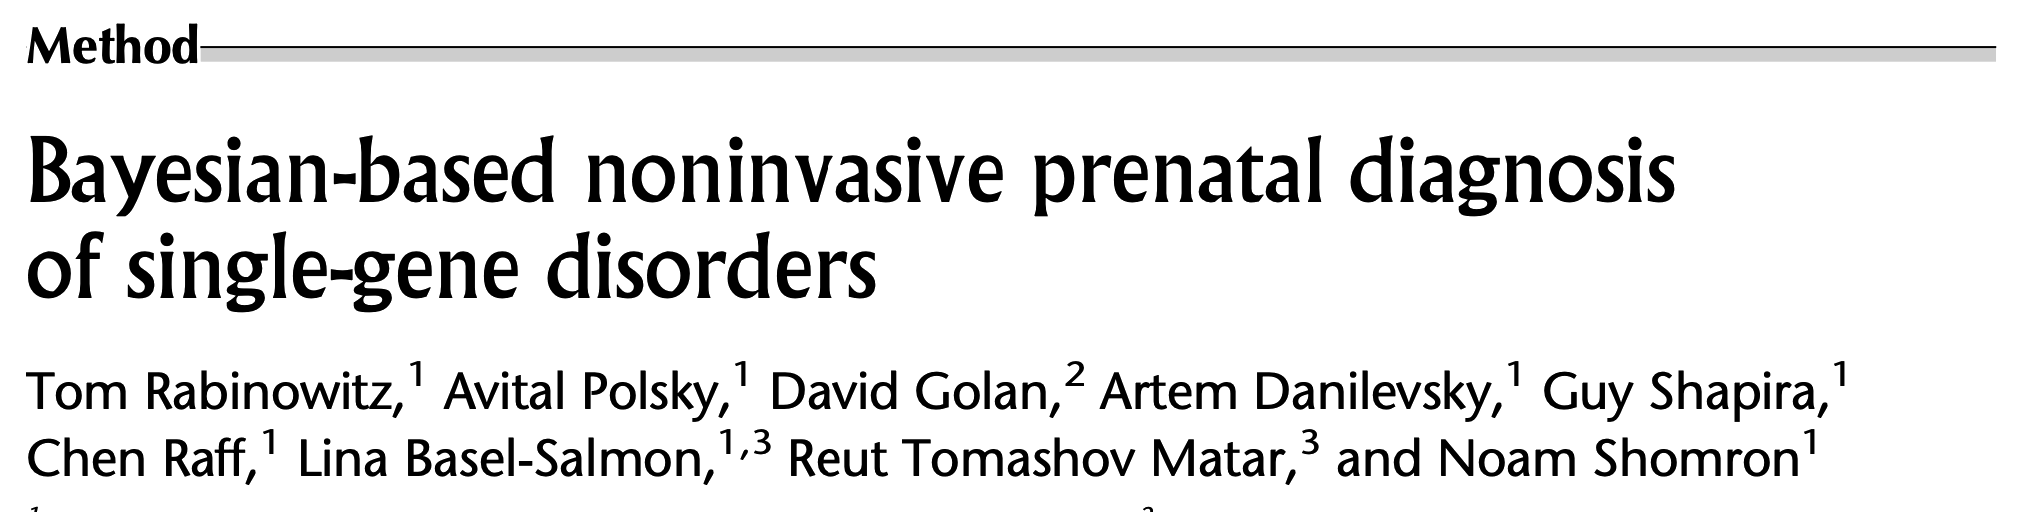
\includegraphics{images/rabinowitz.png}

\end{frame}

\begin{frame}{Does fragment length matter?}
\protect\hypertarget{does-fragment-length-matter-1}{}

\begin{center}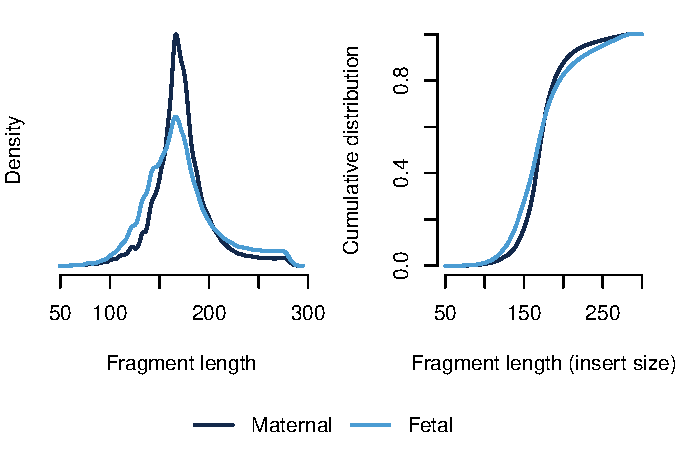
\includegraphics{defense_files/figure-beamer/matVsFetLen-1} \end{center}

\end{frame}

\begin{frame}{Does fragment length matter?}
\protect\hypertarget{does-fragment-length-matter-2}{}

\begin{center}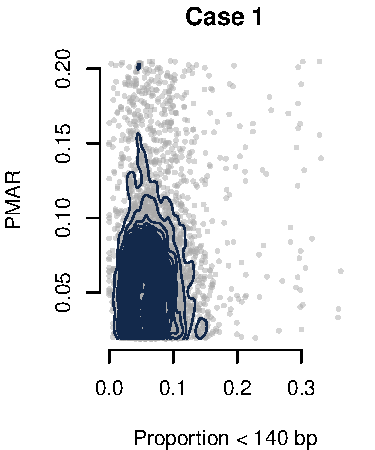
\includegraphics[width=0.32\linewidth]{defense_files/figure-beamer/sratioByPmar-1} 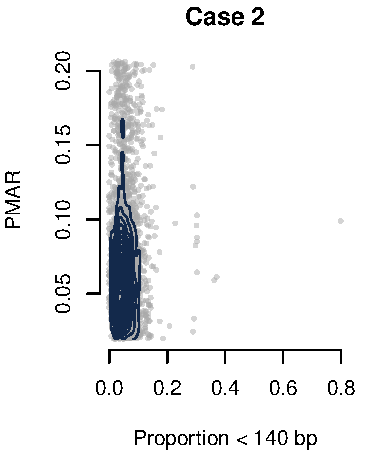
\includegraphics[width=0.32\linewidth]{defense_files/figure-beamer/sratioByPmar-2} 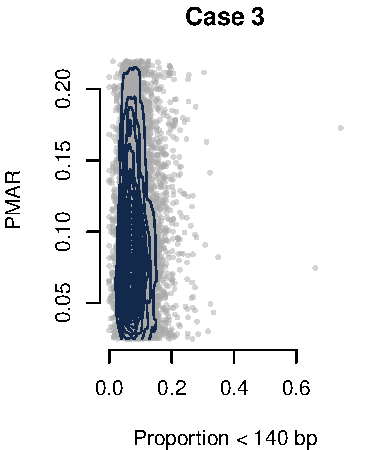
\includegraphics[width=0.32\linewidth]{defense_files/figure-beamer/sratioByPmar-3} \end{center}

\bigskip

\begin{itemize}
\item
  Rabinowitz et al.~found the difference in accuracy varied from -0.25\%
  to 1.89\% when using versus not using fragment length in their exome
  analyses.
\item
  Correcting for fragment length will not overcome the bounds of the
  binomial distribution
\end{itemize}

\end{frame}

\begin{frame}{Summary}
\protect\hypertarget{summary}{}

\begin{itemize}
\item
  Noninvasive exome sequencing would require cost-prohibitive sequencing
  depths
\item
  Despite suggestions by others, simply correcting for fragment length
  will not facilitate noninvasive genome/exome sequencing in the clinic
\item
  We recommend a more targeted approach
\end{itemize}

\end{frame}

\hypertarget{acknowledgments}{%
\subsection*{Acknowledgments}\label{acknowledgments}}
\addcontentsline{toc}{subsection}{Acknowledgments}

\begin{frame}{Acknowledgments}

\begin{minipage}[t]{0.49\linewidth}
\begin{itemize}\scriptsize
  \item Kirk Wilhelmsen
  \begin{itemize}\scriptsize
    \item Fenshen Kuo
    \item Chris Bizon
    \item Jeff Tilson
    \item Darius Bost
    \item Kimberly Robasky
    \item Phil Owen
  \end{itemize}
  \item Thesis Committee
  \begin{itemize}\scriptsize
    \item Bradford Powell (Chair)
    \item Stan Ahalt
    \item Yun Li
    \item Neeta Vora
  \end{itemize}
  \item Jonathan Berg
  \begin{itemize}\scriptsize
    \item Christian Tilley
    \item Alicia Brandt
  \end{itemize}
\end{itemize}
\end{minipage}
\begin{minipage}[t]{0.49\linewidth}
\begin{itemize}\scriptsize
  \item UNC Genetics/BCB
  \begin{itemize}\scriptsize
    \item Will Valdar
    \item Tim Elston
    \item Jonathan Cornett
    \item Cara Marlow
    \item Fernando Pardo-Manuel de Villena
  \end{itemize}
  \item MD/PhD Program
  \begin{itemize}\scriptsize
    \item Toni Darville
    \item Mohanish Deshmuk
    \item Alison Reagan
    \item Carol Herrion
    \item Amber Brosius
  \end{itemize}
\end{itemize}
\end{minipage}

\bigskip

\centering


\includegraphics[height=4em]{images/renci-logo_grey.pdf} \hspace{2ex}
\includegraphics[height=3em]{images/SOM_gray.pdf}

\appendix

\end{frame}

\hypertarget{appendix}{%
\section*{Appendix}\label{appendix}}
\addcontentsline{toc}{section}{Appendix}

\begin{frame}{Appendix}
\protect\hypertarget{appendix-1}{}

\label{apptoc}

\tableofcontents

\end{frame}

\hypertarget{produce-simulated-exomes}{%
\subsection{Produce simulated exomes}\label{produce-simulated-exomes}}

\begin{frame}{Produce simulated exomes}

\medskip

We use an alternate definition of copy state, such that 1 represents the
normal diploid state. Let \(N\) represent the total number of molecules
(read pairs) and \(e_j \in \mathbb{E}\) represent the probability of
capturing target \(j\), then for each subject, \(i\):

\begin{enumerate}
\item
  Randomly select \(s_{ij} \in \mathbb{S}_i\) from
  \(S = \{0.0, 0.5, 1, 1.5, 2\}\) as the copy number at target \(j\)
\item
  Adjust the subject-specific capture probabilities by the copy number,
  \(\mathbb{E}_i = \frac{\mathbb{E} \odot \mathbb{S}_{i}}{\sum_j \mathbb{E} \odot \mathbb{S}_{i}}\)
\item
  Draw \(N\) times from \(\text{Multinomial}(\mathbb{E}_i)\), giving the
  molecule counts at each target \(j\) for sample \(i\),
  \(c_{ij} \in \mathbb{C}_i\)
\end{enumerate}

\end{frame}

\hypertarget{mccnv-algorithm-1}{%
\subsection{mcCNV algorithm}\label{mccnv-algorithm-1}}

\begin{frame}{mcCNV algorithm}

The mcCNV algorithm adjusts the sSEQ probability model by adding a
multiplier for the copy state: \[
  C_{ij} \sim \mathcal{NB}(f_is_{ij}\hat\mu_j, \tilde\phi_j/f_i)
\] where the random variable \(C_{ij}\) represents observed molecule
counts for subject \(i\) at target \(j\), \(f_i\) is the size factor for
subject \(i\), \(s_{ij}\) is the copy state, \(\mu_j\) is the expected
mean under the diploid state at target \(j\), and \(\tilde\phi_j\) is
the shrunken phi at target \(j\). We observe \(c_{ij}\) and wish to
estimate \(s_{ij}\), \(\hat{s}_{ij}\).

\end{frame}

\begin{frame}{mcCNV algorithm}
\protect\hypertarget{mccnv-algorithm-2}{}

Initialize by setting \(\hat{s}_{ij} = 1\) for all \(i,j\). Then,

\begin{enumerate}
\item
  Adjust the observed values for the estimated copy-state, \[
    c_{ij}^{\prime} = \frac{c_{ij}}{\hat{s}_{ij}}.
    \]
\item
  Subset \(c_{ij}^{\prime}\) such that
  \(c_{ij}^{\prime} > 10, ~ \hat{s}_{ij} > 0\)
\item
  Calculate the size-factor for each subject \[
    f_i = \text{median}\left(\frac{c_{ij}^{\prime}}{g_j}\right),
    \] where \(g_j\) is the geometric mean at each exon.
\item
  Use method of moments to calculate the expected dispersion \[
    \hat\phi_j = \max\left(0, \frac{\hat\sigma_j^2 - \hat{\mu}_j}{\hat{\mu}_j^2}\right)
    \] where \(\hat{\mu}_j\) and \(\hat{\sigma}_j^2\) are the sample
  mean and variance of \(c_{ij}^{\prime}/f_i\).
\end{enumerate}

\end{frame}

\begin{frame}{mcCNV algorithm}
\protect\hypertarget{mccnv-algorithm-3}{}

\begin{enumerate}
\setcounter{enumi}{4}
\tightlist
\item
  Let \(J\) represent the number of targets. Shrink the phi values to \[
    \tilde\phi_j = (1 - \delta)\hat\phi_j + \delta\hat{\xi}
    \] such that \[
    \delta = \frac{\sum\limits_j\left(\hat\phi_j - \frac{1}{n_j}\sum\limits_j \hat\phi_j\right)^2/(J - 1)}
    {\sum\limits_j\left(\hat\phi_j - \hat{\xi}\right)^2/(n_j - 2)}
    \] and \[
    \hat{\xi} = \mathop{\text{argmin}}\limits_{\xi}\left\{
    \frac{d}{d\xi}\frac{1}{\sum\limits_j \left(\hat\phi_j - \xi\right)^2}
    \right\}.
    \]
\end{enumerate}

\end{frame}

\begin{frame}{mcCNV algorithm}
\protect\hypertarget{mccnv-algorithm-4}{}

\begin{enumerate}
\setcounter{enumi}{5}
\item
  Update \(\hat{s}_{ij}\), \[
    \mathop{\text{argmax}}\limits_{s \in S}\left\{
    \mathcal{L}(s \rvert c_{ij},f_i,\hat\mu_j,\tilde\phi_j)
    \right\}
    \] where \(S = \{0.001, 0.5, 1, 1.5, 2\}\).
\item
  Repeat until the number of changed states falls below a threshold or a
  maximum number of iterations is reached.
\item
  After convergence, calculate p-values for the diploid state,
  \(\pi_{ij} = \text{Pr}(s_{ij} = 1)\).
\item
  Adjust p-values using the Benjamini--Hochberg procedure and filter to
  a final call-set such that adjusted p-values fall below some
  threshold, \(\alpha\).
\end{enumerate}

\end{frame}

\hypertarget{venn-diagrams-with-all-samples}{%
\subsection{Venn diagrams with all
samples}\label{venn-diagrams-with-all-samples}}

\begin{frame}{Venn diagrams with all samples}

\begin{center}\includegraphics[width=0.49\linewidth]{defense_files/figure-beamer/vennAll-1} \includegraphics[width=0.49\linewidth]{defense_files/figure-beamer/vennAll-2} \end{center}

\centering \includegraphics{defense_files/figure-beamer/vennLgnd-1.pdf}

\end{frame}

\hypertarget{aglient-capture-versus-idt-capture}{%
\subsection{Aglient capture versus IDT
capture}\label{aglient-capture-versus-idt-capture}}

\begin{frame}{Aglient capture versus IDT capture}

\begin{center}\includegraphics{defense_files/figure-beamer/mnVrComp-1} \end{center}

\end{frame}

\hypertarget{maternal-fetal-genotyping-algorithm}{%
\subsection{Maternal-fetal genotyping
algorithm}\label{maternal-fetal-genotyping-algorithm}}

\begin{frame}{Maternal-fetal genotyping algorithm}

Represent maternal and fetal genotype pairs, given by the random
variable \(G\), with capital and lowercase letters, where `A' and `B'
represent the major and minor alleles (e.g.~`AAab' represents the fetus
uniquely heterozygous for the minor allele).

Let \(X,Y\) be random variables for major and minor allele read counts.
Define the fetal fraction and PMAR as the random variables \(F\) and
\(M\).

We employ an empirical Bayesian expectation-maximization algorithm to
identify loci with unique fetal heterozygosity,
i.e.~\(g \in \{\text{AAab}, \text{BBab}\}\). We pick reasonable starting
values for the fetal fraction, \(F = f\), and the average minor allele
frequency, then iteratively update the expected allele distribution and
expected PMAR values until some convergence:

\end{frame}

\begin{frame}{Maternal-fetal genotyping algorithm}
\protect\hypertarget{maternal-fetal-genotyping-algorithm-1}{}

\begin{enumerate}
\item
  Initialize the genotype probabilities, \(p_g^* = \text{Pr}\{G = g\}\),
  and the expected PMAR, \(m_g^* = m_g\), based on reasonable estimates
  for the average minor allele frequency and fetal fraction
\item
  Update \(\hat{\mathbb{G}}\): \[
   \hat{g}_i = \mathop{\text{argmax}}\limits_{g \in G}\left\{p_g^*\mathcal{L}(g \rvert m_g^*,x_i,y_i)\right\}, Y_{i} \sim \text{Bin}(x_i + y_i, m_g^*) 
    \]
\item
  Update the genotype probabilities: \[
   p_g^* = \frac{\sum_i \text{I}(\hat{g} = g) + N\text{Pr}\{G = g\} - 1}{\sum_g\left\{\sum_i \text{I}(\hat{g} = g) + N\text{Pr}\{G = g\} - 2\right\}}
    \] where \(N\) is the weight given to the initial estimate of the
  genotype probability, \(\text{Pr}\{G = g\}\).
\end{enumerate}

\end{frame}

\begin{frame}{Maternal-fetal genotyping algorithm}
\protect\hypertarget{maternal-fetal-genotyping-algorithm-2}{}

\begin{enumerate}
\setcounter{enumi}{3}
\item
  Update the expected PMAR: \[
   m_g^* = \frac{\sum_i y_i\text{I}(\hat{g} = g) + Nm_g - 1}{\sum_i(x_i + y_i)\text{I}(\hat{g} = g) + N - 2} 
    \] where \(N\) is the weight given to the initial estimate of the
  PMAR, \(m_g\).
\item
  Continue updating \(\hat{\mathbb{G}}\) , \(p_g^*\), and \(m_g^*\)
  until \(\hat{\mathbb{G}}\) converges.
\item
  For all loci \(j\), such that
  \(\hat{g} \in \{\text{AAab}, \text{BBab}\}\), calculate \(\hat{f}_j\):
  \[
  \hat{f}_j =
    \begin{cases}
      \displaystyle\frac{2y_j}{x_j + y_j}, & \hat{g} = AAab \\[15pt]
      2 - \displaystyle\frac{2y_j}{x_j + y_j}, & \hat{g} = BBab
    \end{cases} 
    \]
\end{enumerate}

\end{frame}

\begin{frame}{Maternal-fetal genotyping algorithm}
\protect\hypertarget{maternal-fetal-genotyping-algorithm-3}{}

\begin{enumerate}
\setcounter{enumi}{6}
\item
  Let \[
  \hat{f} = \text{median}\left(\hat{f}_j\right)
    \]
\item
  Calculate the expected PMAR using the fetal fraction estimate, \[
   m_g = \text{E}[M|\hat{f},g]
    \]
\item
  Finally, for all loci, \(i\), estimate
  \(\hat{g}_i \in \hat{\mathbb{G}}\), \[
    \hat{g}_i = \mathop{\text{argmax}}\limits_{g \in G}\left\{\mathcal{L}(g \rvert m_g,x_i,y_i)\right\}, Y_{i} \sim \text{Bin}(x_i + y_i, m_g)
    \]
\end{enumerate}

\end{frame}

\hypertarget{all-case-3-calls}{%
\subsection{All case 3 calls}\label{all-case-3-calls}}

\begin{frame}{All case 3 calls}

\begin{minipage}{0.49\linewidth}
\begin{table}[H]
\centering
\begin{tabular}{>{}lllr}
\toprule
Mat & Fet & Cff & N\\
\midrule
\cellcolor{uncgray}{} &  & 0/0 & 468\\

\cellcolor{uncgray}{} & \multirow{-2}{*}{\raggedright\arraybackslash 0/0} & 0/1 & 1,159\\

\cellcolor{uncgray}{} & \cellcolor{gray85}{} & \cellcolor{gray85}{0/0} & \cellcolor{gray85}{64}\\

\cellcolor{uncgray}{} & \cellcolor{gray85}{\multirow{-2}{*}{\raggedright\arraybackslash 0/1}} & \cellcolor{gray85}{0/1} & \cellcolor{gray85}{352}\\

\cellcolor{uncgray}{} &  & 0/0 & 1\\

\cellcolor{uncgray}{\multirow{-6}{*}{\raggedright\arraybackslash 0/0}} & \multirow{-2}{*}{\raggedright\arraybackslash 1/1} & 0/1 & 2\\
\cmidrule{1-4}
\cellcolor{uncgray}{} &  & 0/1 & 1\\

\cellcolor{uncgray}{} & \multirow{-2}{*}{\raggedright\arraybackslash 0/0} & 1/1 & 2\\

\cellcolor{uncgray}{} & \cellcolor{gray85}{} & \cellcolor{gray85}{0/0} & \cellcolor{gray85}{3}\\

\cellcolor{uncgray}{} & \cellcolor{gray85}{} & \cellcolor{gray85}{0/1} & \cellcolor{gray85}{1,308}\\

\cellcolor{uncgray}{} & \cellcolor{gray85}{\multirow{-3}{*}{\raggedright\arraybackslash 0/1}} & \cellcolor{gray85}{1/1} & \cellcolor{gray85}{648}\\

\cellcolor{uncgray}{} &  & 0/1 & 1,601\\

\cellcolor{uncgray}{\multirow{-7}{*}{\raggedright\arraybackslash 1/1}} & \multirow{-2}{*}{\raggedright\arraybackslash 1/1} & 1/1 & 23\\
\bottomrule
\end{tabular}
\end{table}
\end{minipage}
\begin{minipage}{0.49\linewidth}
\begin{table}[H]
\centering
\begin{tabular}{>{}lllr}
\toprule
Mat & Fet & Cff & N\\
\midrule
\cellcolor{uncgray}{} &  & 0/0 & 387\\

\cellcolor{uncgray}{} &  & 0/1 & 107\\

\cellcolor{uncgray}{} & \multirow{-3}{*}{\raggedright\arraybackslash 0/0} & 1/1 & 6\\

\cellcolor{uncgray}{} & \cellcolor{gray85}{} & \cellcolor{gray85}{0/0} & \cellcolor{gray85}{3,072}\\

\cellcolor{uncgray}{} & \cellcolor{gray85}{} & \cellcolor{gray85}{0/1} & \cellcolor{gray85}{1,967}\\

\cellcolor{uncgray}{} & \cellcolor{gray85}{\multirow{-3}{*}{\raggedright\arraybackslash 0/1}} & \cellcolor{gray85}{1/1} & \cellcolor{gray85}{713}\\

\cellcolor{uncgray}{} &  & 0/0 & 68\\

\cellcolor{uncgray}{} &  & 0/1 & 458\\

\cellcolor{uncgray}{\multirow{-9}{*}{\raggedright\arraybackslash 0/1}} & \multirow{-3}{*}{\raggedright\arraybackslash 1/1} & 1/1 & 1,291\\
\bottomrule
\end{tabular}
\end{table}
\end{minipage}

\end{frame}

\end{document}
